\documentclass[12pt]{article}
\usepackage[utf8]{inputenc}
\usepackage{alphabeta}
\usepackage{ dsfont }
\usepackage{parskip}
\usepackage{fullpage}
\usepackage{tikz}
\usepackage{comment}
\usepackage{amssymb}
\usepackage{amsmath}
\usepackage{listings}
\usepackage{etoolbox}
\usepackage[T1]{fontenc}
\usepackage{booktabs}
\usepackage{svg}


\title{\Large Εθνικό Μετσόβιο Πολυτεχνείο \\
Σχολή Ηλεκτρολόγων Μηχανικών \& Μηχανικών Υπολογιστών\\
Επεξεργασία Φωνής και Φυσικής Γλώσσας\\
3ο Εργαστήριο \begin{figure}[h]
\centering

\includegraphics[width=0.2\textwidth]{ntua.jpg}
\end{figure}
}
\author{ \Large  Δωροθέα Καλλιώρα  ΑΜ: 03115176\\ \\
     \Large  Νικήτας Θεοδωρόπουλος AM: 03115185}
\date{Ακαδημαϊκό έτος 2019-2020 - 9ο Εξάμηνο}


\begin{document}
\maketitle
\begin{center}
\end{center}
\bigbreak
\vspace{.5em} \hrule \vspace{.2em} \hrule


\section{Εισαγωγή}


Στόχος της παρούσας εργαστηριακής άσκησης είναι να υπλοποιήσουμε μοντέλα για την επεξεργασία και την κατηγοριοποίηση κειμένων με χρήση Deep Neural Networks DNNs, και την βιβλιοθήκη PyTorch. Για κάθε δείγμα εισόδου σε μορφή κειμένου δημιουργούμε διανυσματικές αναπαραστάσεις με χρήση pretrained word embeddings λέξεων. Συγκεκριμένα χρησιμοποιήσαμε GloVe[2] Twitter (2B tweets, 27B tokens, 1.2M vocab, uncased, 50d,), με σκοπό να αξιοποιήσουμε την πληροφορία συναισθήματος στα tweets για το δέυτερο dataset που περιέχονται στα emojis, σημεία στίξης κτλπ. 

Στόχος είναι να εκπαιδεύσουμε μοντέλα τα οποία θα μπορούν να κάνουν ανάλυση συναισθήματος (sentiment analysis) σε προτάσεις. 

\begin{itemize}
    \item \textbf{Sentence Polarity Dataset} [Pang and Lee, 2005][3] To dataset περιέχει 5331 θετικές και 5331 αρνητικές κριτικές ταινιών, από το Rotten Tomatoes και είναι binary-classification πρόβλημα (positive, negative).
    \item \textbf{Semeval 2017} Task4-A [Rosenthal et al.,2017][4]. To dataset αυτό περιέχει tweets τα οποία είναι κατηγοριοποιημένα σε 3 κλάσεις (positive, negative,neutral) με 49570 παραδείγματα εκπαίδευσης και 12284 παραδείγματα αξιολόγησης.
\end{itemize}


\section{Προπαρασκευή}


\textbf{1: Προεπεξεργασία των δεδομένων:}

Αρχικά έγινε κατάλληλη προεπεξεργασία των δεδομένων με χρήση των κλάσεων Dataset, Dataloader. Τα labels αντιστοιχίζονται σε αριθμούς και στα κείμενα γίνεται κατάλληλο tokenization και αντιστοίχιση των λέξεων σε embeddings indexes. Χρησιμοποιηθήκε ο NLTK sentence tokenizer. 

Για να μπορέσει να γίνει επεξεργασία των δεδομένων θα πρέπει τα δέιγματα να έχουν το ίδιο μέγεθος για τον λόγο αυτό επιλέχθηκε το σταθερό μέγεθος 60 λέξεων, και έγινε κατάλληλο padding ή μείωση. Το πραγματικό μήκος αποθηκεύεται. Τα δεδομένα μετατρέπονται σε Tensors απο την κλάση Dataloader

\textbf{2: Μοντέλο}

Σχεδιάζουμε την αρχιτεκτονική του Νευρωνικού Δικτύου. Με χρήση ενός embedding layer δημιουργούμε μια συνεχή διανυσματική αναπαράσταση για κάθε όρο της πρότασης, και για το δυνολικό δείγμα λαμβάνοντας τον μέσο όρο. Ο μέσος όρος προκύπτει διαιρώντας το άθροισμα με το πραγματικό μήκος του κειμένου, (τα embeddings των padded elements αντιστοιχίζονται στο μηδενικό διάνυσμα).

Το embedding layer όπως έχουμε δει αντιστοιχίζει κοντα λέξεις που είναι σημασιολογικά κοντά. Τα embeddings αρχικοποιούνται με τα pretrained GloVe embeddings. Και έπειτα παγώνουν $(requires\_grad=False)$.

Τα διανύσματα προβάλονται απο το embedding layer μέσω μιας μη γραμμικής συνάρτησης ενεργοποίησης (ReLU) σε έναν ενδιάμεσο χώρο 100 διαστάσεων. Το τελευταίο layer προβάλει τα διανύσματα στον χώρο εξόδου. Για Binary Classification επιλέχθηκε output layer μεγέθους 1, για compatibillity με το BCELoss. Για την κατηγοριοποίηση τριών κλάσεων έγινε αντιστοίχιση $\mathbb{R}^{100} \rightarrow \mathbb{R}^3$.

Υλοποιούμε το Forward pass εφαρμόζοτας σε κάθε mini-batch τους παραπάνω μετασχηματισμούς. 

\textbf{3: Εκπαίδευση}

Τα παραδέιγματα οργανώνονται σε mini-batches μεγέθους 128. Μεγαλύτερη τιμή είναι προτιμότερη για το Semeval2017A dataset λόγω του μεγάλου αριθμού δεδομένων. Εκτελούμε σε κάθε βήμα Stochasitc Gradient Descend. 

Για την εκπαίδευση χρησιμοποιούμε τα εξής:

\begin{itemize}
    \item \textbf{Κριτήριο:} \textbf{BCEWithLogitsLoss} για δεδομένα 2 κλάσεων. \textbf{CrossEntropyLoss} για δεδομένα 3 κλάσεων. 
    \item \textbf{Παράμετροι:} Το learning rate επιλέχθηκε $lr = 0.0001$, διότι παρατηρήσαμε οτι μεγαλύτερες τιμές οδηγούν σε μεγάλωσες ταλαντωσεις του loss και μειώνουν την απόδοση. Οι παράμετροι των μοντέλων με $requires\_grad=True$ βελτιστοποιούνται με Gradient Descend
    \item \textbf{Optimizer:} Επιλέγουμε \textbf{Adam} καθώς χρησιμοποιείται ευρέως στην βιβλιογραφία και έχει γενικά καλα αποτελέσματα. Επίσης προσαρμόζει αυτόματα την ταχύτητα ενημέρωσης των μαρών.
\end{itemize}

Αξιολογούμε το μοντέλο στο τέλος κάθε εποχής, εκτυπώνοντας το train loss. Παρακάτω για τα δύο Data sets εκπαιδεύουμε τα μοντέλα και παρουσιάζουμε τα τελικά αποτελέσματα: 

\begin{figure}[h!]
	\centering
	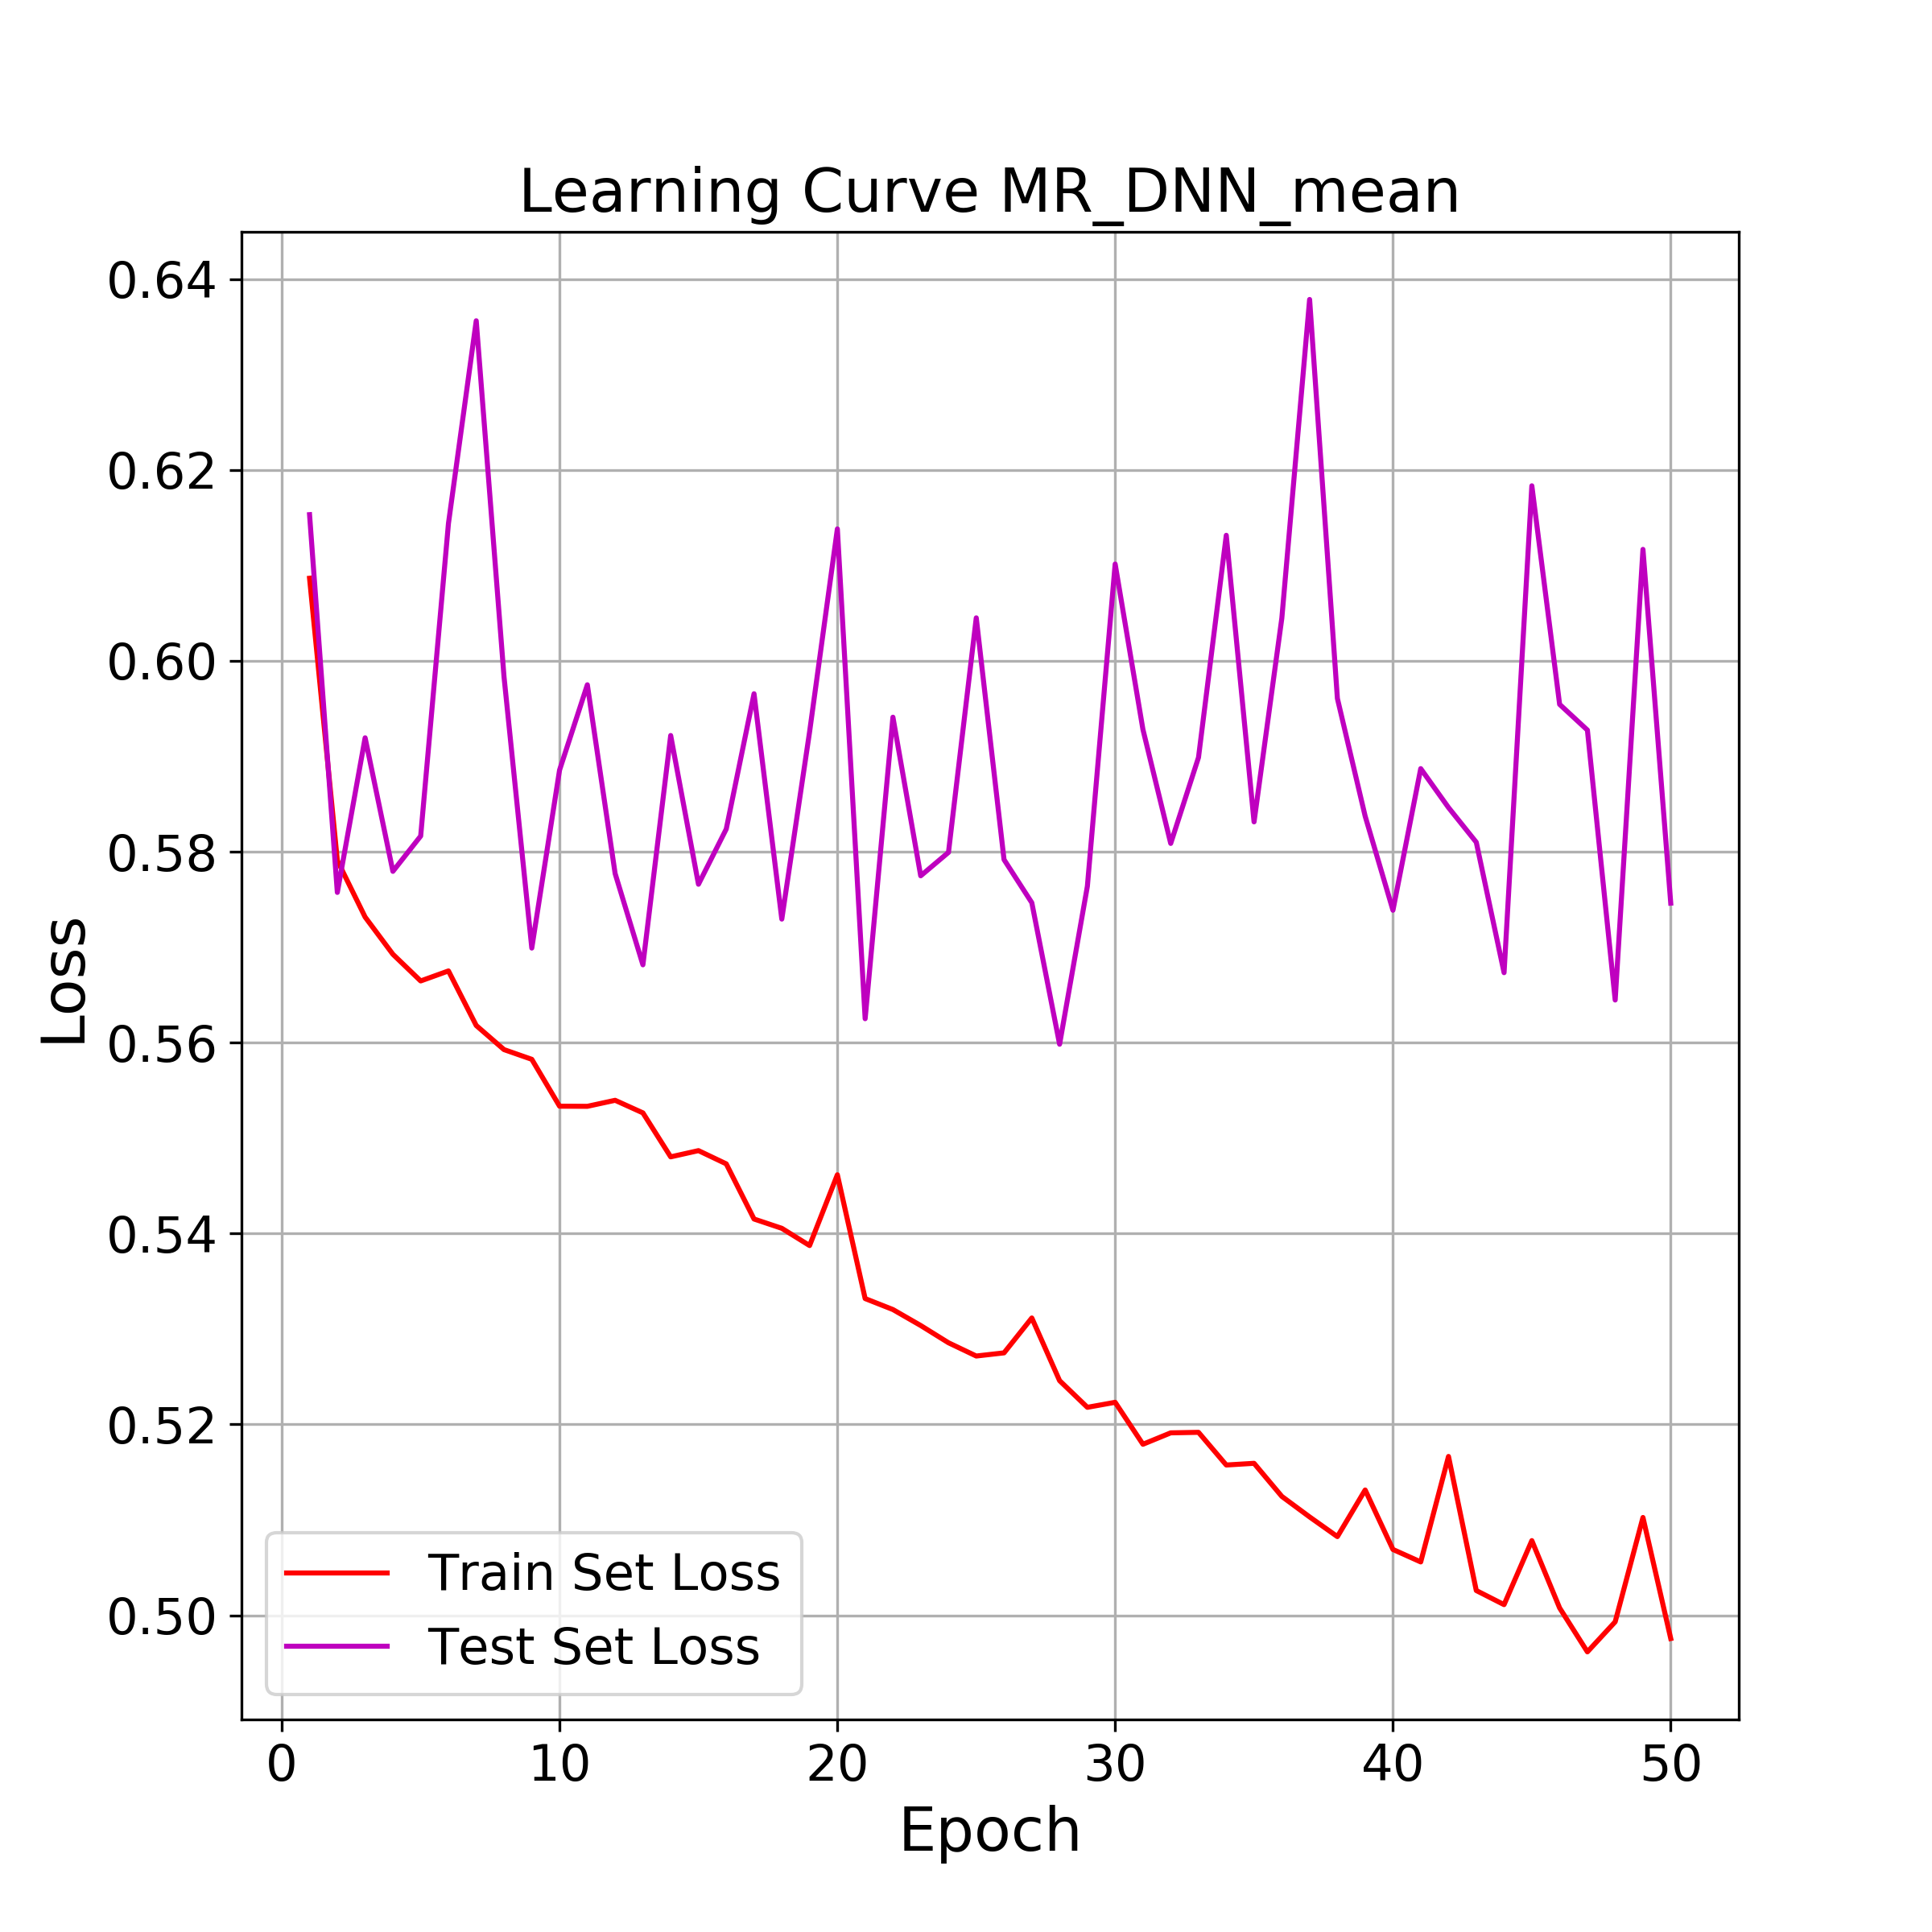
\includegraphics[width=0.5\linewidth]{./img/MR/DNN_mean_loss}
	\caption{Learning Curve - MR}
	\label{fig:sin}
\end{figure}


\begin{figure}[h!]
	\centering
	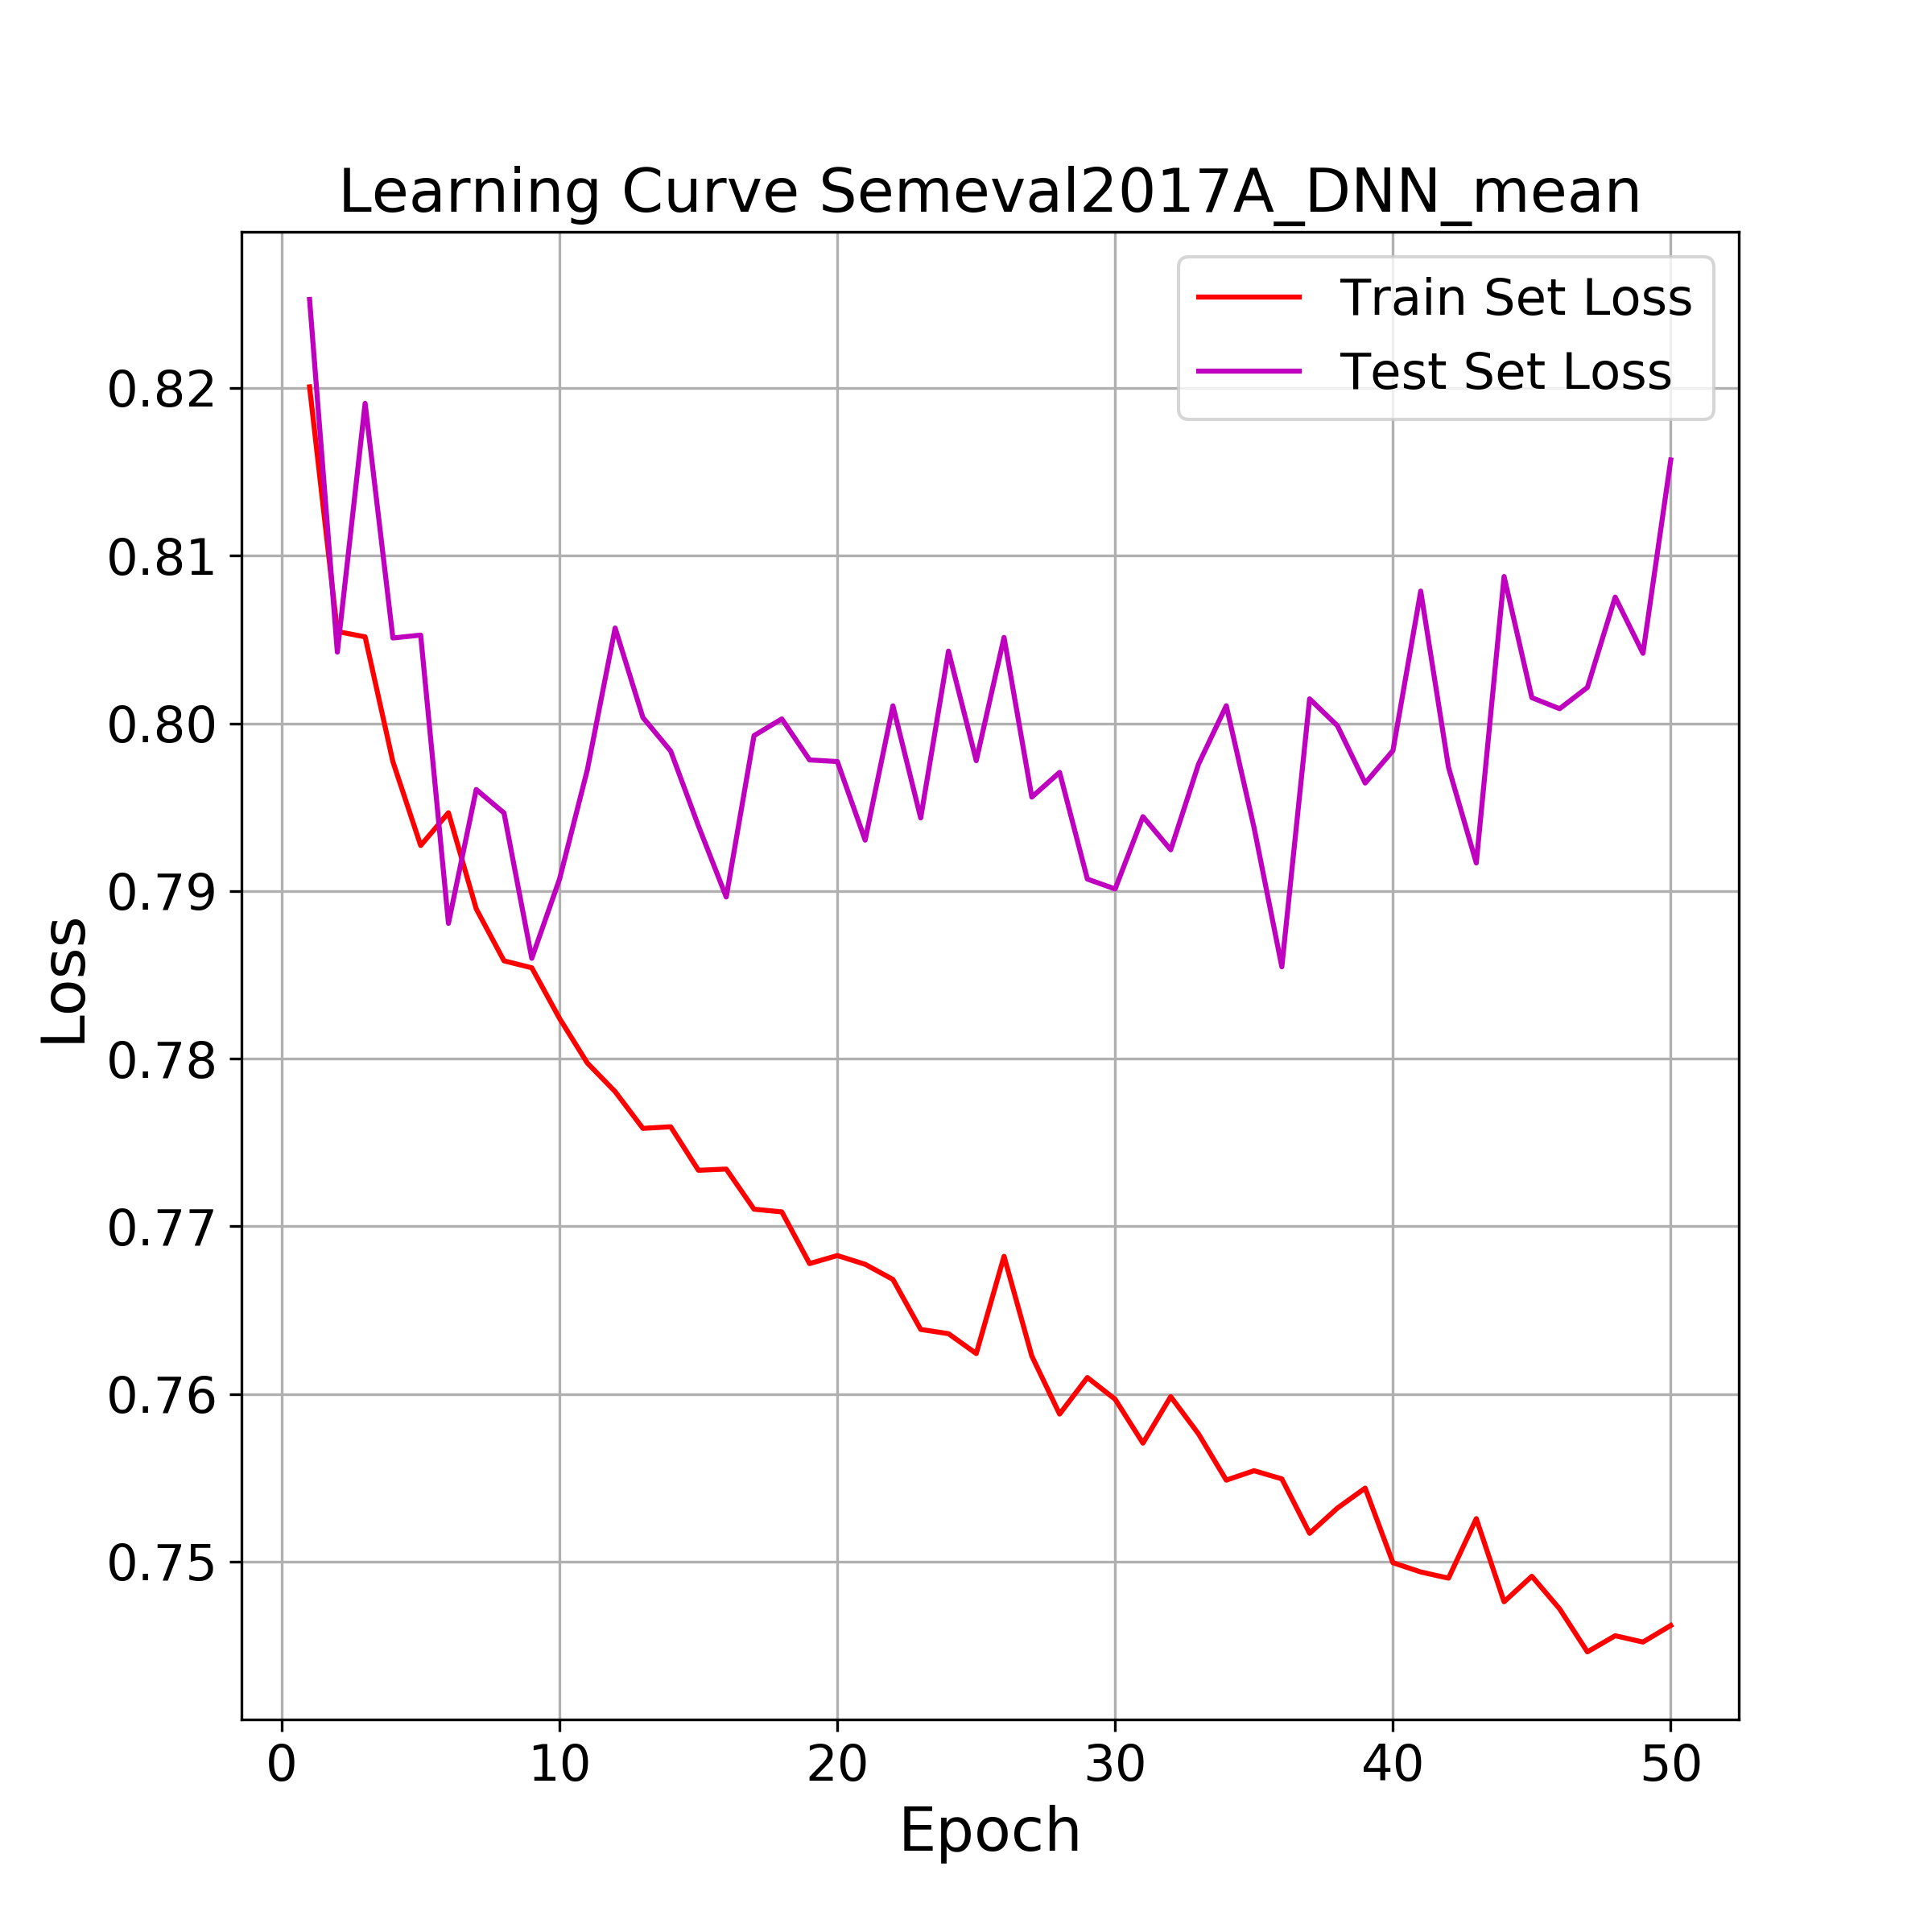
\includegraphics[width=0.5\linewidth]{./img/Semeval2017A/DNN_mean_loss}
	\caption{Learning Curve - Semeval2017A}
	\label{fig:sin}
\end{figure}




\textbf{Απαντήσεις ερωτημάτων}

\textbf{Ερώτημα 1:Γιατί αρχικοποιούμε το embedding layer με τα προ-εκπαιδευμένα word embeddings;}

Για την αρχικοποίηση των βαρών του embedding layer είχαμε δύο επιλογές: να χρησιμοποιήσουμε βάρη απο pre-trained word embeddings ή να αρχικοποιήσουμε τα βάρη σε τυχαίες τιμές οι οποίες θα μαθαίνονταν κατά την εκπαίδευση του μοντέλου. Επιλέξαμε να χρησιμοποιήσουμε τα βάρη των pre-trained word embedding. 


Τα pre-trained embeddings αναπαριστούν τις λέξεις σε ένα διανυσματικό χώρο ώστε οι σημασιολογικά κοντινές λέξεις να έχουν μικρή απόσταση. Η εκπαίδευση τους έχει γίνει σε corpus εκατομμυρίων λέξεων, και αποτελούν ένα τεράστιο λεξικό αναπαραστάεων. 

Κείμενα με κοντινή αναπαράσταση στον embedded χώρο θα έχουν και κοντινό συναισθηματικό περιεχόμενο και άρα θα πρέπει να δώσουν κοινή έξοδο. Η πληροφορία αυτή ειναι ανεκτίμητη για έναν ταξινομητή συναισθήματος, και προφανώς δε μπορεί να συναχθεί απο τα δεδομένα εκπαίδευσης στον ίδιο βαθμό. Ακόμα οδηγούν σε καλύτερο generalization αφού λέξεις του test set μπορεί να διαθέτουν pre-trained embedding αλλα να μην γίνονται γνωστές απο το train set. 

Συμπερασματικά τα embeddings περιέχουν πλούσια σημασιολογική πληροφορία  και το DNN θα μπορέσει να αξιοποιήσει τις αναπαραστάσεις για να έχει καλύτερη απόδοση και να συγκλίνει πιο γρήγορα. 

\textbf{Ερώτηση 2: Γιατί κρατάμε παγωμένα τα βάρη του embedding layer κατά την εκπαίδευση;}

Οι λόγοι που κρατάμε παγωμένα τα βάρη του embedding layer κατά την εκπαίδευση είναι οι εξής:

\begin{itemize}
    \item Τα βάρη που προκύπτουν από τα pre-trained word embeddings έχουν δημιουργηθεί από ένα μεγάλου μεγέθους corpus και δείχνουν μια συσχέτιση μεταξύ των λέξεων. Η συσχέτιση αυτή, μαθαίνεται μετά από την εκπαίδευση σε high-end μηχανές και χρησιμοποιώντας βέλτιστες παραμέτρους. Άρα, δεν χρειάζεται περαιτέρω ανανέωση των τιμών των βαρών με αποτέλεσμα να μειώνεται η υπολογιστή πολυπλοκότητα του αλγορίθμου.
    \item Αν συνεχίσουμε να ανανεώνουμε τις τιμές των βαρών των pre-trained word embeddings κατά την εκπαίδευση, ενδέχεται να αλλάξουμε τις συσχετίσεις που δείχνουν αρχκά τα embeddings και να μην έχουμε την επιθυμητή συμπεριφορά από το emdedding layer. Συγκεκριμένα, μια ανεπιθύμητη συμπεριφορά είναι το overfitting του DNN. Αν συνεχιστεί η ανανέωση των βαρών, το DNN θα εκπαιδευτεί πολύ καλά πάνω στο training set που έχουμε και έτσι δεν θα έχει καλή απόδοση σε κάποιο άλλο dataset.
\end{itemize}

\textbf{Ερώτηση 3: Γιατί βάζουμε μία μη γραμμική συνάρτηση ενεργοποίησης στο προτελευταίο layer; Τι διαφορά θα είχε αν είχαμε 2 ή περισσότερους γραμμικούς μετασχηματισμούς στη σειρά;}

Οποιαδήποτε λειτουργία θέλουμε να κάνει το νευρωνικό δίκτυο που δημιουργούμε θέλουμε να την αναπαραστήσουμε σε μία υπολογιστική συνάρτηση.Για να πετύχουμε αυτό θα πρέπει να εφαρμόσουμε μια συνάρτηση ενεργοποίησης $f(x)$ έτσι ώστε το δίκτυο να γίνει πιο ισχυρό, να έχει την ικανότητα να μαθαίνει κάτι περίπλοκο και πολύπλοκο από τα δεδομένα και να αναπαριστά μη γραμμικές σύνθετες και αυθαίρετες αντιστοιχίες μεταξύ εισόδου και εξόδου. Ως εκ τούτου, χρησιμοποιώντας μη γραμμική ενεργοποίηση, είμαστε σε θέση να παράγουμε μη γραμμικές απεικονίσεις από τις εισόδους στις εξόδους αφού οι μη γραμμικές συναρτήσεις έχουν βαθμό μεγαλύτερο από ένα και έχουν καμπυλότητα όταν τις σχεδιάζουμε. Για προβλήματα classification πρέπει να μπορούμε να υπολογίσουμε μη γραμμικά decision boundaries.

Αν δεν είχαμε χρησιμοποιήσει μη-γραμμική συνάρτηση ενεργοποίησης, όσα layers και να βάζαμε στο DNN μας, θα συμπεριφερόταν σαν ένα single-layer perceptron αφού αν αθροίζαμε όλα τα layers του θα παίρναμε μια συνολική γραμμική συνάρτηση. Άρα, το μοντέλο θα προσπαθούσε κάθε φορά να αντιστοιχίσει την είσοδο με την έξοδο γραμμικά 
και έτσι θα είχαμε μία πολύ απλή αναπαράσταση των δεδομένων.  

\textbf{Ερώτηση 4: Αν θεωρήσουμε ότι κάθε διάσταση του embedding χώρου αντιστοιχεί σε μία αφηρημένη έννοια, μπορείτε να δώσετε μία διαισθητική ερμηνεία για το τι περιγράφει η αναπαράσταση που φτιάξατε(κέντρο-βάρους).}

Θεωρούμε έναν χώρο όπου κάθε διάσταση αντιστοιχίζεται και σε μία αφηρημένη έννοια. Τοτε για ένα διάνυσμα του χώρου $x = (x_1,x_2,...,x_n)$ η τιμή $x_i$ του διανύσματος εκφράζει την συσχέτιση με την έννοια της διάστασης $i$, πόσο κοντά δηλαδή σημασιολογικά είναι το κείμενο με την έννοια. Κάθε λέξη του κειμένου αποτελεί και ένα διάνυσμα που έχει μεγαλύτερη τιμή σε άλλες διάστασεις. Κάθε τιμή του μέσου όρου μας δίνει μια μετρική για το πόσο κοντά ειναι το κείμενο με την συγκεκριμένη έννοια. Για χαμηλές τιμές το κείμενο είναι ασυσχέτιστο με τις έννοιες και για υψηλές τιμές η συσχέτιση είναι μεγάλη. 

\textbf{Ερώτηση 5: Αναφέρετε πιθανές αδυναμίες της συγκεκριμένης προσέγγισης για να αναπαραστήσουμε κείμενα.}

\begin{itemize}
    \item Στη συγκεκριμένη προσέγγιση δεν λαμβάνουμε υπόψιν την θέση της λέξης. Η σημασιολογία μίας λέξης αλλάζει ανάλογα με την θέση της στην πρόταση, και μια αρνητική λέξη μπορεί να μετατραπεί σε θετική σε διαφορετικά συμφραζόμενα. Ένας τρόπος να αντιμετοπιστεί αυτο το πρόβλημα είναι με εισαγωγή n-gram language models παράλληλα με τα embeddings.
    \item Ακόμα, δεν λαμβάνουμε υπόψιν την σύνταξη της πρότασης, αφού αθροίζουμε απλά τις λέξεις χωρίς να ελέγχουμε για άλλα στοιχεία της πρότασης και τον  ρόλο λέξεων. 
    \item Τέλος, τα σημεία στίξης του κειμένου δεν επηρεάζουν την αναπαράσταση. Τα σημεία στίξης προσδίδουν διαφορετικό νόημα σε κάθε λέξη και δείχνουν διαφορετικό συναίσθημα για κάθε πρόταση.
\end{itemize}

\textbf{Ερώτηση 6: Τι συνέπειες έχουν τα μικρά και μεγάλα mini-batches στην εκπαίδευση των μοντέλων;}

Για αρκετά μεγάλο batch size μπορούμε να πετύχουμε μια σταθερή εκτίμηση για το ποιο θα είναι το gradient για το συνολικό data set. Ακόμα ανεβαίνει σημαντικά η ταχύτητα εκπαίδευσης αφού το gradient υπολογίζεται αθροιστικά για ένα σύνολο δεδομένων και έπειτα πραγματοποιείται back propagation και gradient descend. Όσο πιο μικρό είναι το batch size τόσο λιγότερη ακριβής ειναι η εκτίμηση. Τα μικρά batches έχουν όμως θόρυβο αφού αποτελούνται από πολλά raw δεδομένα, το οποία μπορεί να βοηθήσει το μοντέλο να ξεφύγει απο τοπικά ελάχιστα και άρα να οδηγήσει σε καλύτερη βελτιστοποίηση. Όταν είναι πολύ μικρό όμως το μοντέλο παρουσιάζει έντονη ταλάντωση ή συγκλίνει πολυ αργά. Μικρά batch sizes μπορούν επίσης να μειώσουν το generalization error. 

Γενικά το σωστό μέγεθος batch είναι σημαντικό γιατί επηρεάζει την ταχύτητα σύγκλισης του μοντέλου, την υπολογιστικη πολυπλοκότητα αλλα και την τελική απόδοση. 

\textbf{Ερώτηση 7: Συνήθως ανακατεύουμε την σειρά των mini-batches στα δεδομένα εκπαίδευσης σε κάθε εποχή. Μπορείτε να εξηγήσετε γιατί;}

Θέλουμε να κάνουμε shuffle τη σειρά των mini-batches δεδομένα εκπαίδευσης για τους παρακάτω λόγους:

\begin{itemize}
    \item Το DNN που έχουμε δημιουργήσει μπορεί εκτός από τις συναρτήσεις ενεργοποίησης που συνδέουν την είσοδο με την έξοδο να μάθει και την σειρά με την οποία δίνονται σε αυτό τα δεδομένα για την εκπαίδευση του. Άρα, αν κάνουμε shuffle ανά εποχή, το νευρωνικό βλέπει κάθε φορά τα δεδομένα με διαφορετική σειρά και δεν μπορεί να κάνει κάποια αντιστοίχιση της εισόδου με την έξοδο βασισμένο αυτή.
    \item Το shuffle των mini-batches ανά εποχή μπορεί επίσης να βοηθήσει το DNN να συγκλίνει πιο γρήγορα στο ολικό ελάχιστο κατά την εκτέλεση του stochastic gradient descent. Αυτό συμβαίνει γιατί αν σε μία εποχή ο αλγόριθμος έχει ‘’κολλήσει’’ σε τοπικό ελάχιστο, στην επόμενη εποχή έχει μεγάλη πιθανότητα να ‘’ξεκολλήσει’’ αφού τα δεδομένα θα δίνονται με διαφορετική σειρά στο νευρωνικό δίκτυο.  
    \item Αν κάνουμε shuffle τη σειρά εισάγουμε τυχαιότητα στη σειρά που δίνονται τα δεδομένα στο δίκτυο ανά εποχή και έτσι το loss που παίρνουμε σαν αποτέλεσμα είναι πιο αμερόληπτο.
\end{itemize}

\textbf{Ερώτηση 8: Αξιολόγηση του ζητούμενου 10}


\begin{tabular}{lrrrr}
\toprule
Semeval2017 DNN\_mean &  precision &    recall &  f1-score &       support \\
\midrule
0            &   0.643151 &  0.550856 &  0.593436 &   3972.000000 \\
1            &   0.621538 &  0.714502 &  0.664786 &   5937.000000 \\
2            &   0.611084 &  0.529263 &  0.567238 &   2375.000000 \\
accuracy     &   0.625773 &  0.625773 &  0.625773 &      0.625773 \\
macro avg    &   0.625258 &  0.598207 &  0.608487 &  12284.000000 \\
weighted avg &   0.626506 &  0.625773 &  0.622855 &  12284.000000 \\
\bottomrule
\end{tabular}

Min Test Loss: 0.785475
\\

\begin{tabular}{lrrrr}
\toprule
MR DNN\_mean &  precision &    recall &  f1-score &    support \\
\midrule
0            &   0.672316 &  0.719033 &  0.694891 &  331.00000 \\
1            &   0.698052 &  0.649547 &  0.672926 &  331.00000 \\
accuracy     &   0.684290 &  0.684290 &  0.684290 &    0.68429 \\
macro avg    &   0.685184 &  0.684290 &  0.683908 &  662.00000 \\
weighted avg &   0.685184 &  0.684290 &  0.683908 &  662.00000 \\
\bottomrule
\end{tabular}

Min Test Loss: 0.559829



Παρατηρούμε ότι οι καμπύλες έιναι φυσιολογικές με το loss να πέφτει και στα δύο σύνολα. Η τιμή learning rate που επιλέξαμε είναι καλή αλλιώς θα βλέπαμε απότομη αύξηση του loss. 

Στο \textbf{MR} dataset παρατηρούμε μεγάλη ταλάντωση του loss function στο test set που σημαίνει οτι δεν γίνεται καλο generalization και απαιτεί περαιτέρω διερεύνηση.  

Στο \textbf{Semeval2017A} η καμπύλη εκπαίδευσης παραπέμπει σε καλά αποτελέσματα, με το loss να πέφτει σταθερά και στα δύο σύνολα. 


Η ακρίβεια είναι \textbf{0.68} και \textbf{0.62} αντίστοιχα. Μεγαλύτερη στο \textbf{MR} όπως περιμένα αφού ειναι ευκολότερο πρόβλημα. Τα f1\_score ως καλύτερες μετρικές απόδοσης ακολουθούν το accuracy. Αναφέρουμε οτι στο \textbf{Semeval2017A} η κλάση 1 (neutral) πάει σημαντικά καλύτερα απο τις άλλες (20\% διαφορά στην ακρίβεια). Ακόμα η κλάση 0 (negative) έχει αρκετά χαμηλή τιμή recall \textbf{0.55}. Για το \textbf{MR} οι μετρικές είναι πολυ καλές.


\section{Θεωρητικό Υπόβαθρο}


\subsection*{RNN-LSTM}
\begin{figure}[h!]
	\centering
	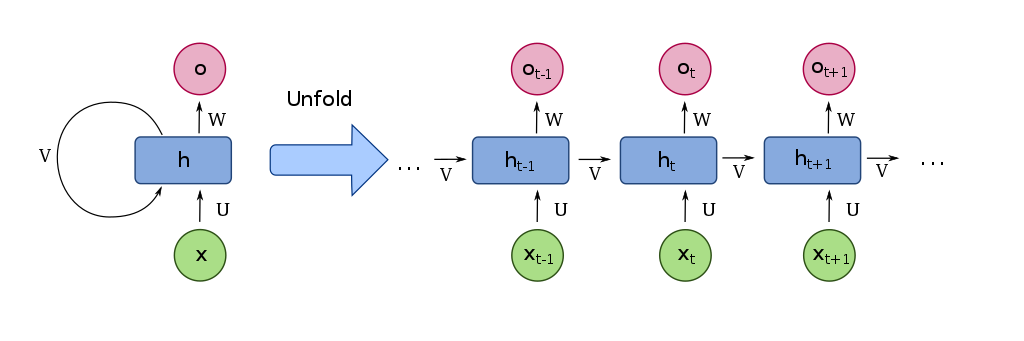
\includegraphics[width=0.6\linewidth]{./img/rnn.svg.png}
	\caption{RNN}
	\label{fig:sin}
\end{figure}


Ένα recurrent neural netword ή RNN είναι μια κλάση νευρωνικών δικτύων με την ικανότητα να χρησιμοποιούν μια εσωστερική κατάσταση (μνήμη) για να εμφανίζουν δυναμική συμπεριφορά.  Είναι φτιαγμένα για επεξεργασία ακολουθιών, και είναι εξαιρετικά για tasks όπως αναγνώριση χειρόγραφων ψηφίων ή φωνής. Εάν ορίσουμε ένα πιο πολύπλοκο δίκτυο με ειδικευμένες πύλες που ελέγχοτν την ροή πληροφορίας προκύπτει τα  Long short-term memmory netowkrs (LSTMs) . Οι πύλες μπορούν να αποφασίσουν ποια πληροφορία ενισχύεται, μεταβάλλεται ή ξεχνιέται απο το ένα κελί στο άλλο.

Τα απλά RNN είναι μια ακολουθία απο layers με σύνδεση μίας κατεύθυνσης. Κάθε νευρώνας έχει μια χρονικά μεταβαλόμενη συνάρτηση ενεργοποίησης, και μεταβαλόμενο βάρος.  Καθώς ξετυλίγεται το μοντέλο στον χρόνο η κρυφή ακολουθία μεταφέρεται απο το ένα κελί στο άλλο προσομοιώνοντας την μνήμη. Τα παραδοσιακά RNN μπορούν να θυμηθούν μεγάλες ακολουθίες αλλα πάσχουν απο προβλήματα vanishing gradients αφού καθώς το gradient ταξιδεύει μέσα απο το κελιά του δικτύου μικραίνει όλο και περισσότερο μέχρι που δεν γίνεται καμία ανανέωση στα βάρη του μοντέλου. Στον αντίποδα είναι το expoding gradient, που οδηγεί σε Overflow. 

\begin{figure}[h!]
	\centering
	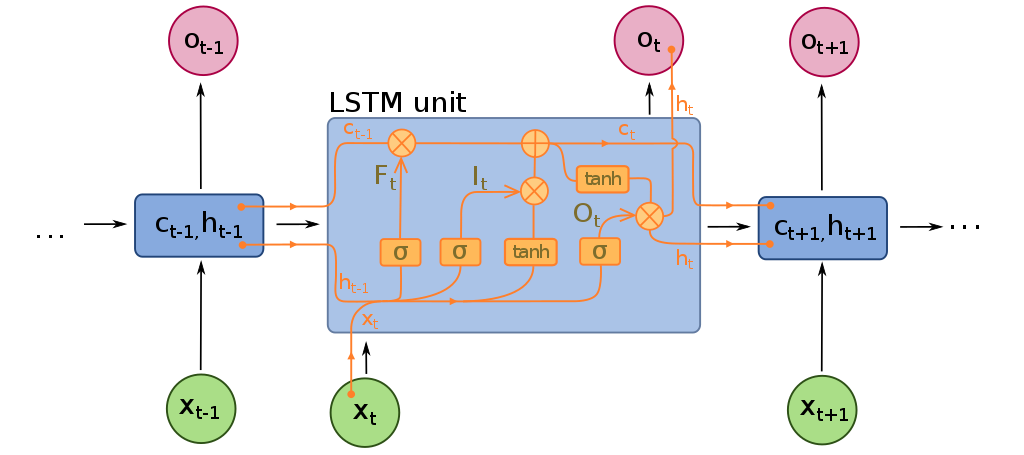
\includegraphics[width=0.6\linewidth]{./img/lstm.png}
	\caption{LSTM architecture}
	\label{fig:sin}
\end{figure}



Μια κοινή αρχιτεκτονική LSTM έχει ένα κελί (μνήμη) με τρείς πύλες που ελέγχουν την ροή της πληροφορίας. Η input gate καθορίζει  εάν μία νέα τιμή μπορέι να εισχωρήσει στο κελί, η  forget gate καθορίζετι το τι μένει, και η πύλη εξόδου καθορίζει το πόσο επηρεάζει την έξοδο του LSTM. 

Τα LSTM έχουν τα παρακάτω πλεονεκτήματα:

1. Αποφεύγουν προβλήματα vanishing  .
2. Ενισχυμένες ικανότητες μνήμης, μπορούν να θυμηθούν εκαττομύρια βήματα πριν.
3. Μπορούν να αναγνωρίσουν context-sensitive γλώσσες.

Μια απλή βελτίωση στα RNN όπως θα δούμε και παρακάτω είναι η χρήση και των δυο κατευθήνσεων της ακολουθίας. Συγκεκριμένα η ακολουθία περνάει απο το RNN/LSTM και απο τις δύο καυεθύνσεις και το τελικό αποτέλεσμα είναι η συνένωση των εξόδων κάθε χρονική στιγμή:

$$h_i = h_i^{\rightarrow} || h_i^{\leftarrow}, h_i \in \mathbb{R}^{2N}$$

Μία αλλη λογική προσέγγιση είναι η αύξηση των επιπέδων, δίνοντας τις εξόδους ενός RNN ως είσοδο σε έαν δεύτερο και παίρνοντας τελικά σαν αποτέλεσμα τις εξόδους του δεύτερου RNN.


\subsection*{Μηχανισμός Προσοχής}

Όπως είδαμε και παραπάνω, ένα RNN χρησιμοποιεί την τελευταία τιμή της εσωτερικής του κατάστασης ως την διανυσματική αναπαράσταση όλης της ακολουθίας. Η αναπαράσταση αυτή ενημερώνεται καθώς το RNN διαβάζει την ακολουθία και στο τέλος περιέχει μία σύνοψη της ακολουθίας. Υπάρχει όμως η περίπτωση το δίκτυο να μην μπορεί να συγκρατήσει όλες τις σημαντικές πληροφορίες στην εσωτερική του κατάσταση. Για να αντιμετω-
πίσουμε το πρόβλημα  μπορούμε να χρησιμοποιήσουμε ένα μηχανισμό προσοχής (attention), ο οποίος επιχειρεί να ενισχύσει την συνεισφορά των
πιο σημαντικών στοιχείων στην τελική αναπαράσταση.

Αυτό το πετυχαίνει αξιοποιώντας όλες τις ενδιάμεσες καταστάσεις του RNN.  Κάθε χρονική στιγμή t, η εσωτερική κατάσταση του RNN y i , χρησιμοποιείται ως την ερμηνεία της λέξης x i , καθώς το RNN κωδικοποιεί κάθε λέξη βάση των συμφραζόμενων. Για την παραγωγή της διανυσματικής
αναπαράστασης ολόκληρου του κειμένου, χρησιμοποιούμε το σταθμισμένο άθροισμα των ερμηνειών των λέξεων με μία πιθανοτική κατανομή $a_i$, $\sum a_i = 1$.



\subsection*{Transfer Learning}
Κατά την διαδικασία Μεταφοράς Γνώσης (Transfer Learning) εκπαιδεύουμε ένα στατιστικό μοντέλο σε ένα πρόβλημα μηχανική μάθησης και το εφαρμόζουμε σε
μια άλλη εφαρμογή. Παρατηρήθηκε ότι τα βάρη δικτύων δικτύων
εκπαιδευμένα σε τεράστια σύνολα δεδομένων για αναγνώρισης εικόνων (ImageNet), μπορούσαν να χρησιμοποιηθούν για την αρχικοποίηση δικτύων με στόχο την επίλυση άλλων προβλημάτων ανάλυσης εικόνας. Τα δίκτυα αυτά είχαν μάθει να αναγνωρίζουν πολύ γενικά χαρακτηριστικά στα χαμηλότερα επίπεδά τους, τα οποία ήταν χρήσιμα σε πολλά διαφορετικά προβλήματα.

Η ίδια προσέγγιση μπορεί να εφαρμοστεί και σε προβλήματα επεξεργασίας φυσικής γλώσσας όταν έχουμε λίγα δεδομένα εκπαίδευσης. Η χρήση προεκπαιδευμένων word embeddings είναι μία
μορφή Μεταφοράς Γνώσης. 




\section{Ερωτήματα}
Στην άσκηση πειραματατιστήκαμε με διαφορετικές αναπαραστάσεις των δεδομένων με χρήση κάθε φορά embeddings. Η ακολουθία x αφου περάσει απο το embedding layer χρησιμοποιείται για τον υπολογισμό μιας εσωτερικής αναπαράστασης. Οι διαφορετικές αναπαραστάσεις έχουν ως σκοπό να αυξήσουν την αναγνωριστική ικανότητα του μοντέλου μας και να μας οδηγήσουν σε καλύτερη απόδοση. 

Για το κύριο μέρος της εργασίας χρησιμοποιήσαμε το dataset $Semeval2017A$.

\subsection{Ερώτημα 1}
\textbf{Ερώτημα 1.1:}
Υπολογίζουμε την αναπαράσταση κάθε πρότασης u σύμφωνα με την σχέση:
$$ E = (e_1,e_2,...,e_N)$$

$$ u = [mean(E)||max(E)]$$
Προκύπτουν τα αποτελέσματα:

\begin{figure}[h!]
	\centering
	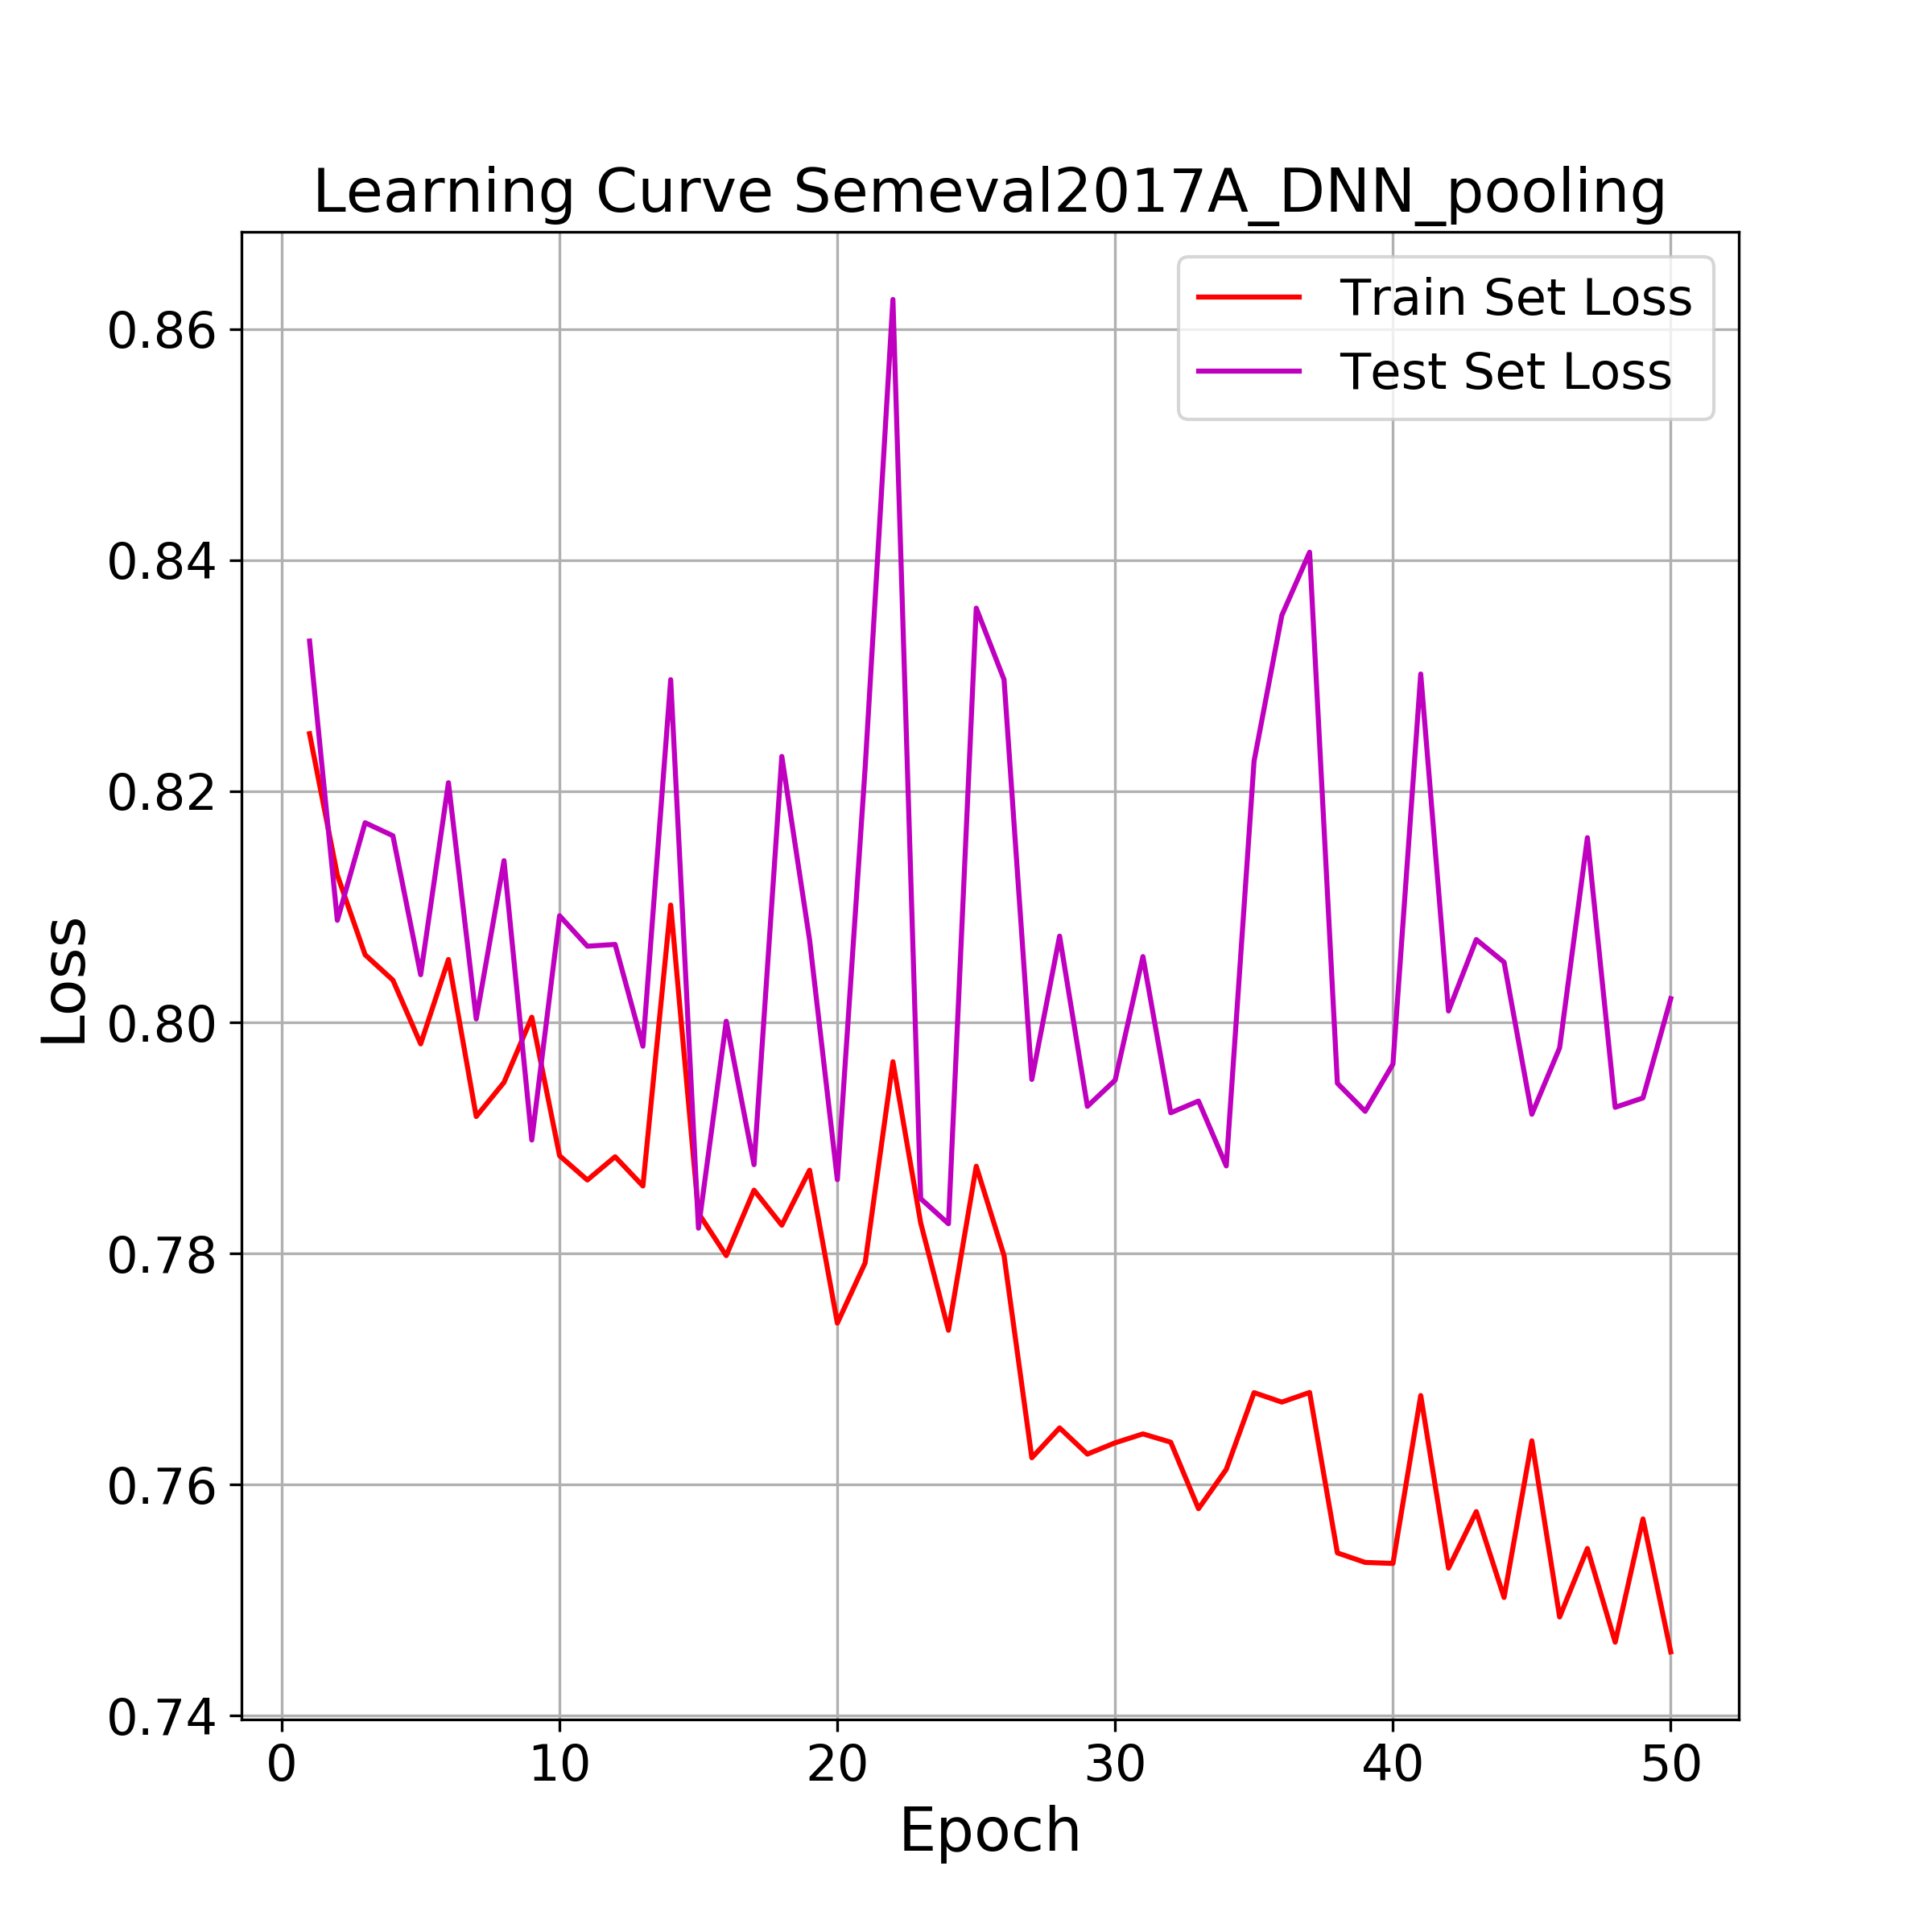
\includegraphics[width=0.6\linewidth]{./img/Semeval2017A/DNN_pooling_loss.png}
	\caption{DNN\_pooling Learning Curve}
	\label{fig:sin}
\end{figure}

\begin{tabular}{lrrrr}
\toprule
DNN\_pooling &  precision &    recall &  f1-score &     support \\
\midrule
0            &   0.620108 &  0.638218 &  0.629032 &   3972.0000 \\
1            &   0.644358 &  0.671383 &  0.657593 &   5937.0000 \\
2            &   0.624876 &  0.528842 &  0.572862 &   2375.0000 \\
accuracy     &   0.633100 &  0.633100 &  0.633100 &      0.6331 \\
macro avg    &   0.629780 &  0.612814 &  0.619829 &  12284.0000 \\
weighted avg &   0.632750 &  0.633100 &  0.631976 &  12284.0000 \\
\bottomrule
\end{tabular}

Min Test Loss: 0.782194



\textbf{Ερώτημα 1.2:}

Στο mean poοling η αναπαράσταση μίας πρότασης προκύπτει ως το μέσο όρο των τιμών των embeddings της κάθε λέξης που απαρτίζει την πρόταση. Αντίθετα, στο max pooling η αναπαράσταση της πρότασης είναι η μέγιστη τιμή των embeddings των λέξεων της πρότασης. Στην πρώτη περίπτωση, θεωρούμε ότι όσο ποιο μεγάλες είναι οι τιμές που έχει κάθε διάσταση της αναπαράστασης u = mean(e1,e2,e3,....,en), E = (e1,e2,e3,....,en) ,τόσο περισσότερο συσχετίζονται οι λέξεις της πρότασης μεταξύ τους. Άρα, πχ αν έχουμε ένα θετικό tweet τότε θα έχει λέξεις που εκράζουν θετικά συναισθήματα. Όμως χρησιμοποιώντας το mean pooling ενδέχεται να μη δοθεί η απαραίτητη σημασιά σε κάποιες λέξεις που μπορεί να αλλάζουν το νόημα όλης της πρότασης και να μην είναι νοηματικά κοντά με τις υπόλοιπες λέξεις. Για παράδειγμα η λέξη 'αλλά' στην πρόταση μπορεί να κάνει ένα tweet neutral αλλά με τη μέση τιμή να φαίνεται ότι είναι αρητικό ή θετικό λόγω των άλλων λέξεων. Για αυτό το λόγο στο Ερώτημα 1 αποφασίσαμε να χρησιμοποιήσουμε το concatεnation της αναπαράστασης του mean pooling με αυτής του max pooling για να πάρουμε τα θετικά και από τις δύο μεθόδους.  



\subsection{Ερώτημα 2}
\textbf{Ερώτημα 2.1:}
Χρησιμοποιούμε τώρα ένα LSTM για την κωδικοποίηση της πρότασης, με είσοδο τα word-embeddings E. Για κάθε λέξη και με γνώση των προηγούμενων παράγει μια αναπαράσταση $h_i$,που λαμβάνει υπόψιν της τα συμφραζόμενα.

\begin{figure}[h!]
	\centering
	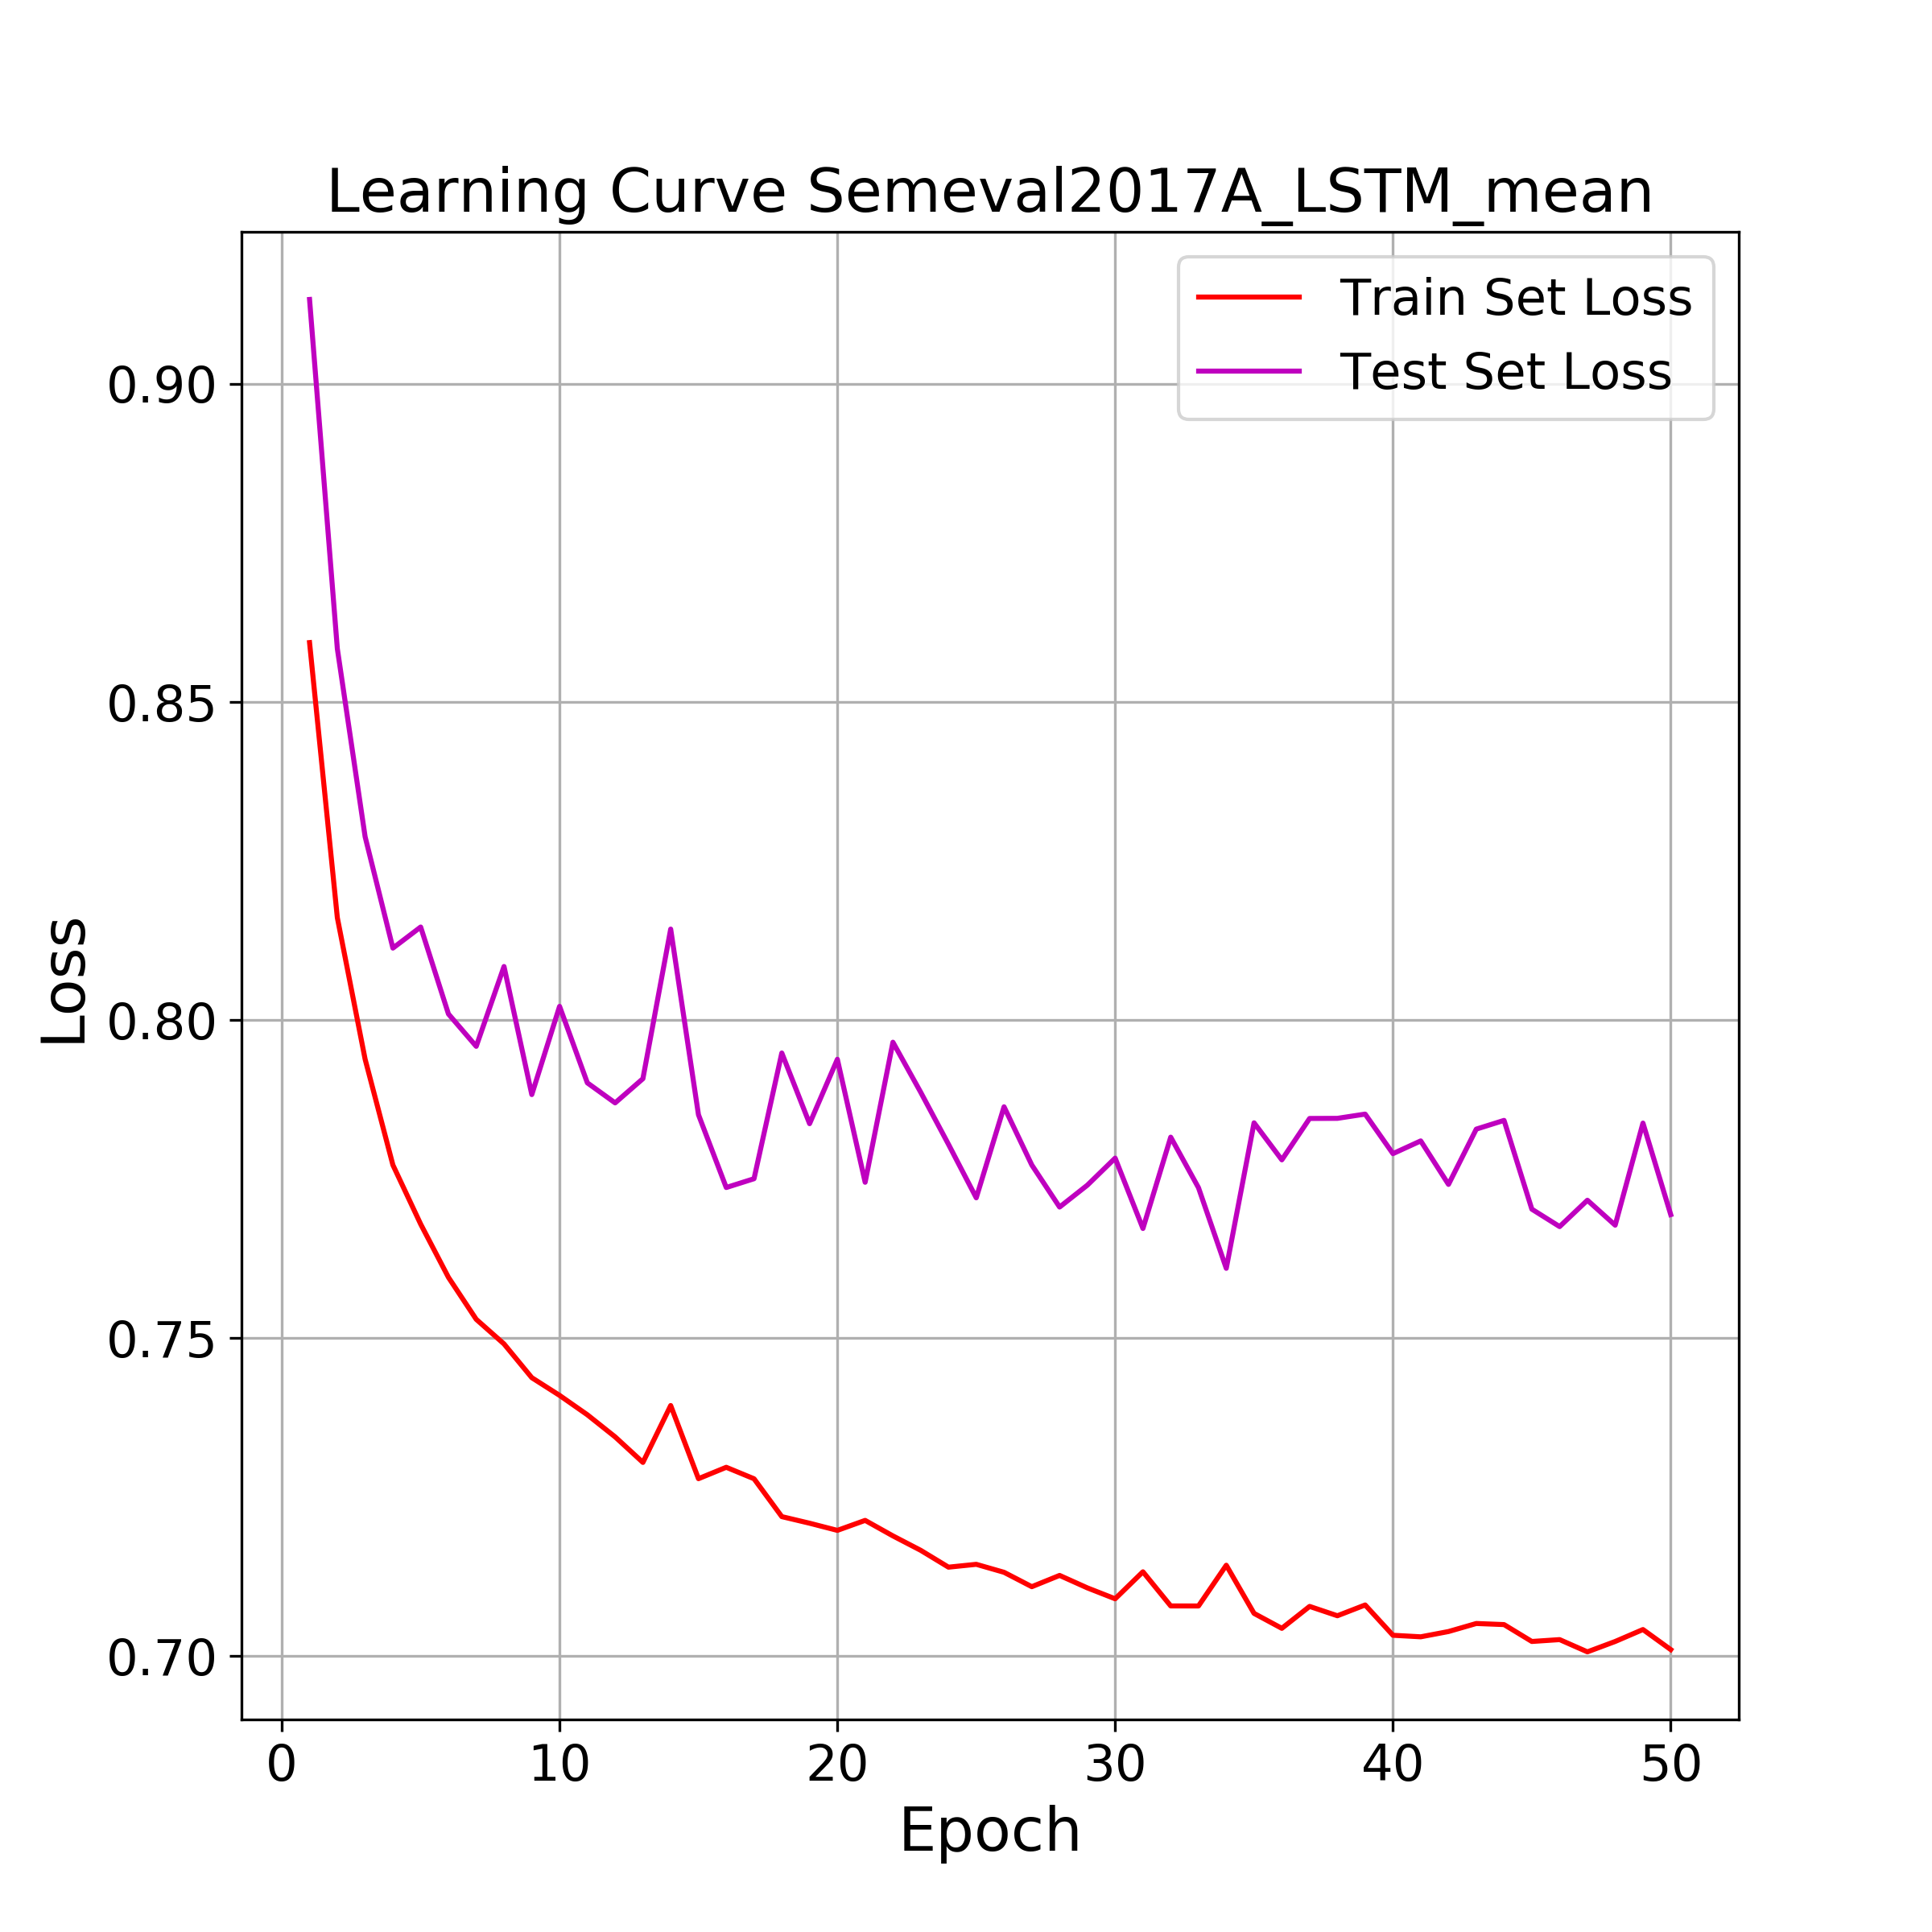
\includegraphics[width=0.6\linewidth]{./img/Semeval2017A/LSTM_mean_loss}
	\caption{LSTM\_mean ($h_i$ as representation) Learning Curve}
	\label{fig:sin}
\end{figure}

\begin{tabular}{lrrrr}
\toprule
LSTM\_mean &  precision &    recall &  f1-score &       support \\
\midrule
0            &   0.677504 &  0.587613 &  0.629365 &   3972.000000 \\
1            &   0.645544 &  0.742968 &  0.690838 &   5937.000000 \\
2            &   0.659521 &  0.557053 &  0.603972 &   2375.000000 \\
accuracy     &   0.656789 &  0.656789 &  0.656789 &      0.656789 \\
macro avg    &   0.660856 &  0.629211 &  0.641392 &  12284.000000 \\
weighted avg &   0.658580 &  0.656789 &  0.654166 &  12284.000000 \\
\bottomrule

Min Test Loss: 0.760955

\end{tabular}

Min Test Loss: 0.760955


\textbf{Ερώτημα 2.2:}
Υπολογίζουμε την εσωτερική αναπαράσταση ως εξής:

$$u = [h_t || mean(E) || max(E)]$$

\begin{figure}[h!]
	\centering
	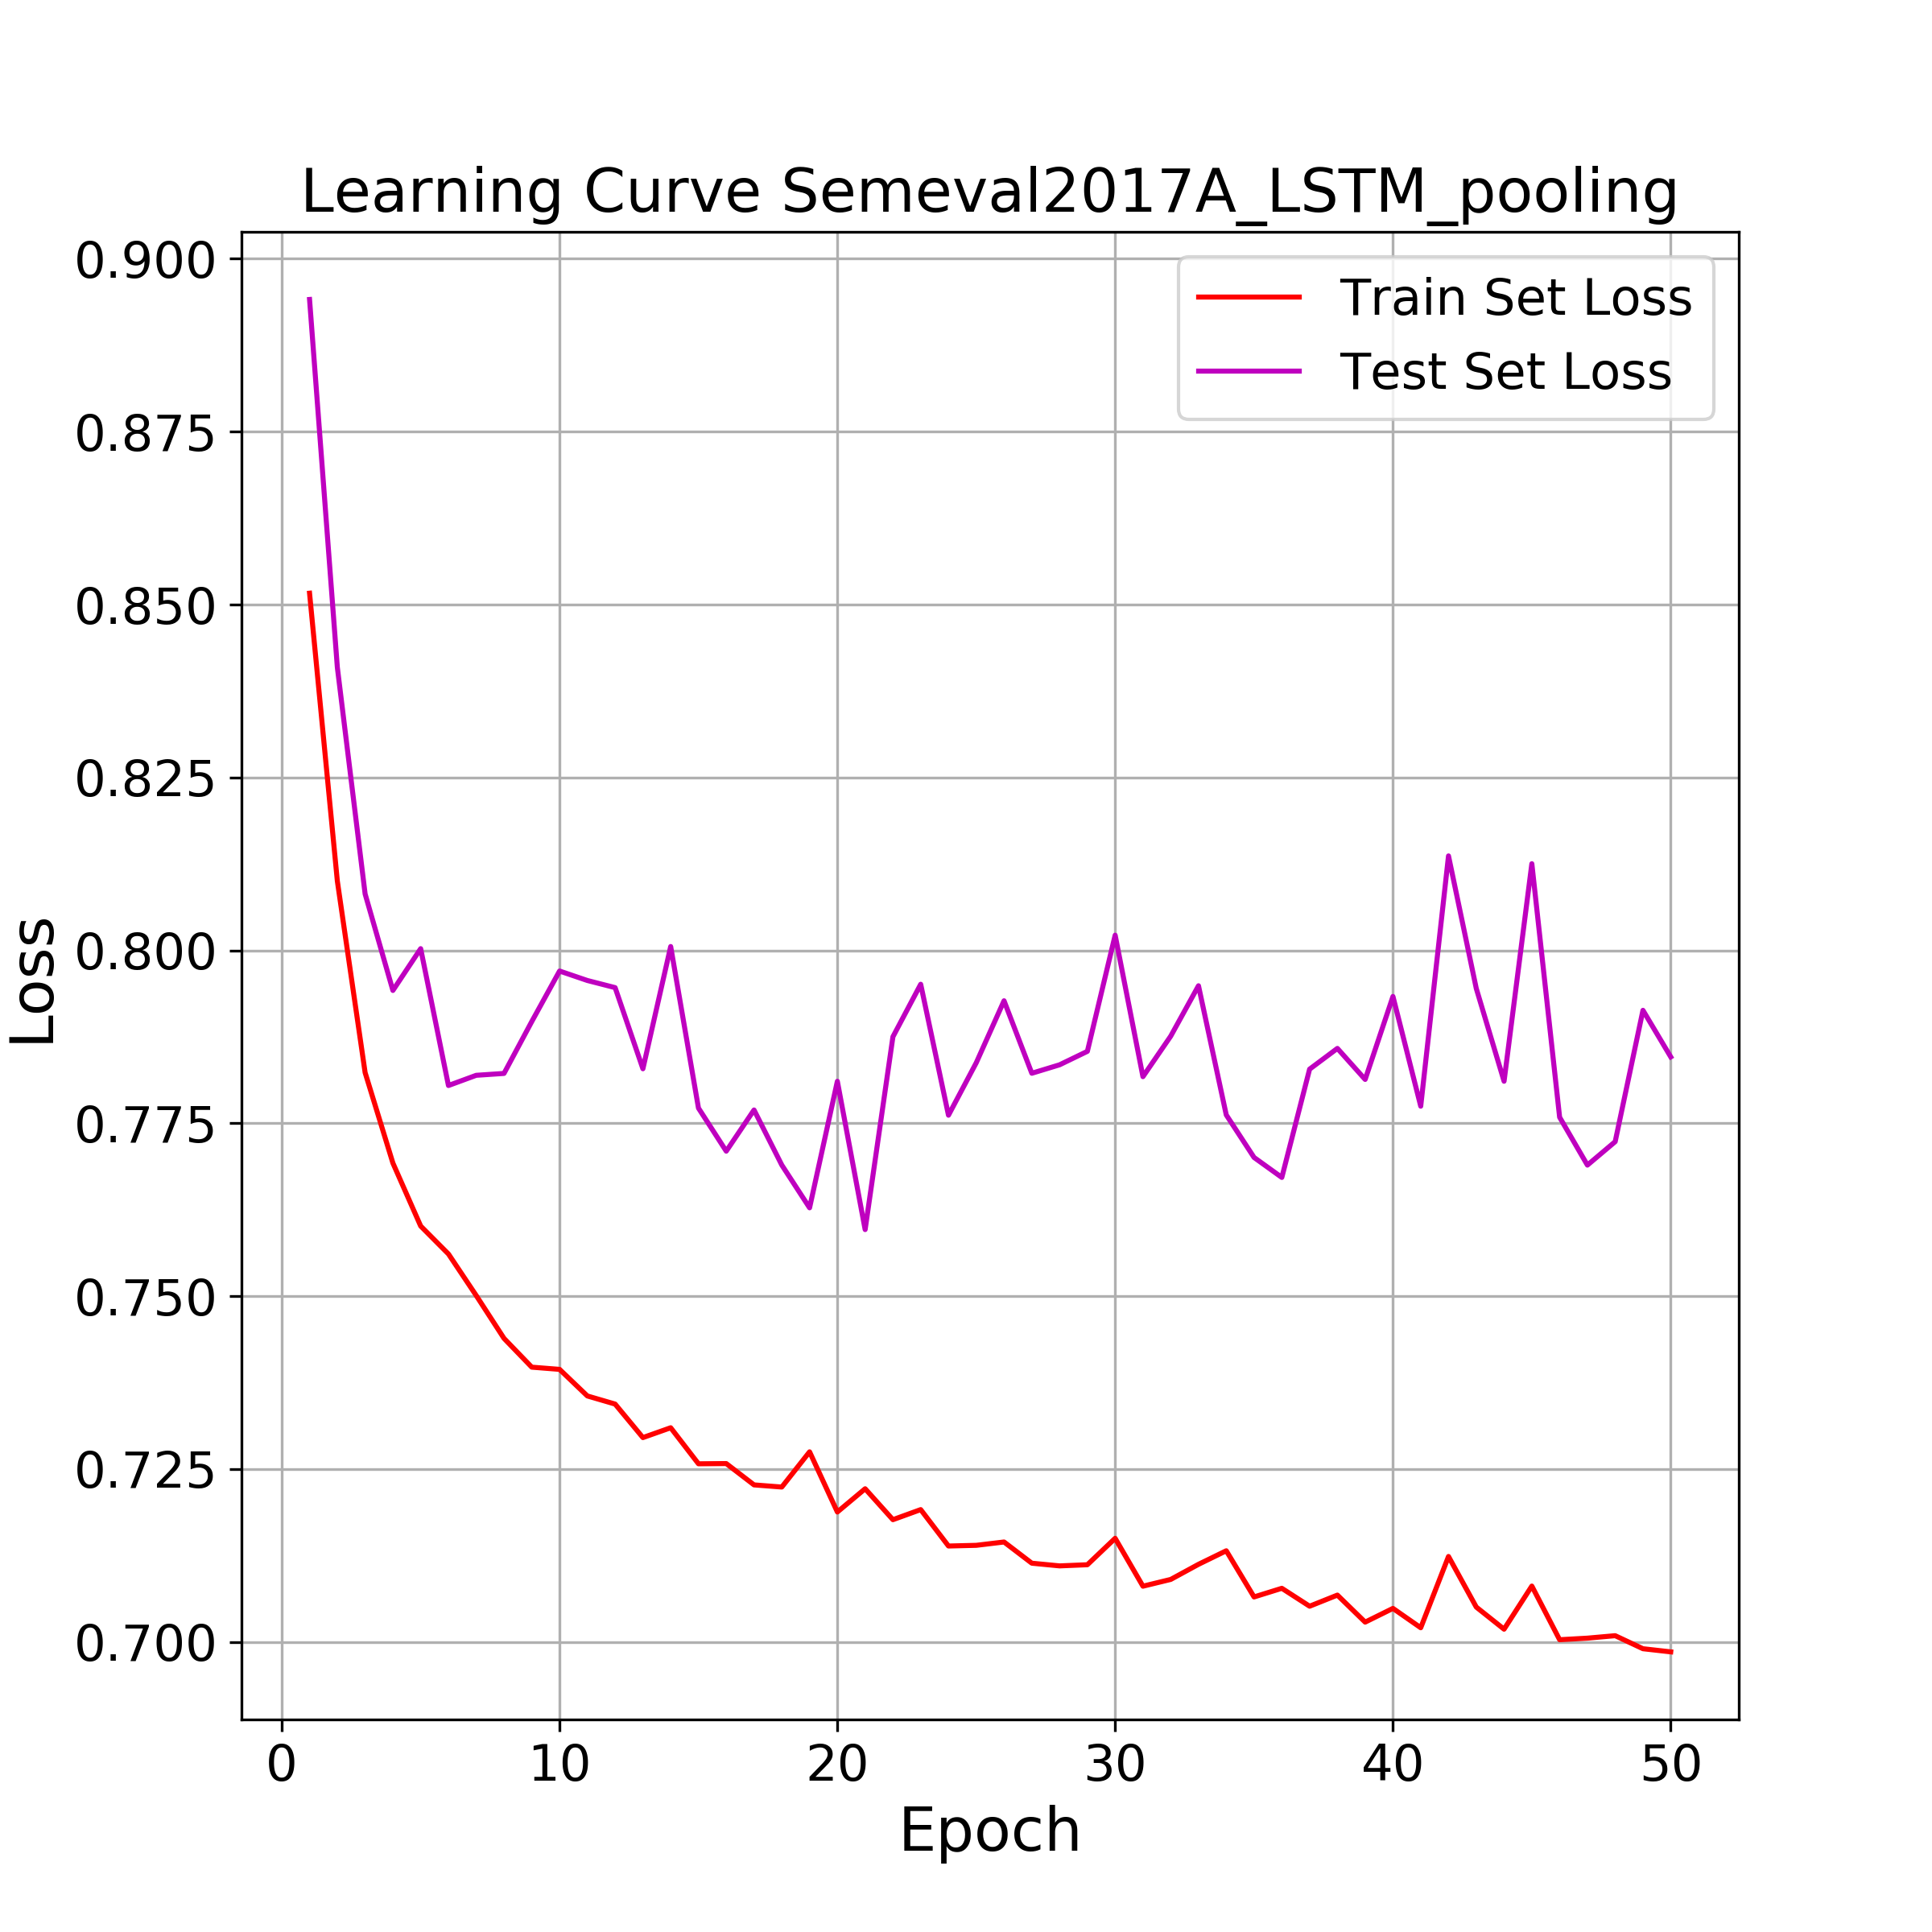
\includegraphics[width=0.6\linewidth]{./img/Semeval2017A/LSTM_pooling_loss.png}
	\caption{LSTM\_pooling Learning Curve}
	\label{fig:sin}
\end{figure}

\begin{tabular}{lrrrr}
\toprule
LSTM\_pooling &  precision &    recall &  f1-score &       support \\
\midrule
0            &   0.656668 &  0.606244 &  0.630449 &   3972.000000 \\
1            &   0.656785 &  0.697827 &  0.676684 &   5937.000000 \\
2            &   0.621048 &  0.603789 &  0.612297 &   2375.000000 \\
accuracy     &   0.650033 &  0.650033 &  0.650033 &      0.650033 \\
macro avg    &   0.644834 &  0.635953 &  0.639810 &  12284.000000 \\
weighted avg &   0.649838 &  0.650033 &  0.649286 &  12284.000000 \\
\bottomrule
\end{tabular}

Min Test Loss: 0.759627




\subsection{Ερώτημα 3}
\textbf{Ερώτημα 3.1:}
Υλοποιούμε έναν μηχανισμό attention σαν ξεχωριστό pytorch module , και έπειτα τον καλούμε στις επιμέρους αρχιτεκτονικές DNN, LSTM.

$$u_i = tanh(W\mathbf{e_i}+b)$$
$$a_i = softmax(u_i)$$
$$u = \sum_{i=1}^N a_i\mathbf{e_i}$$

Τα αποτελέσματα προκύπτουν:


\begin{figure}[h!]
	\centering
	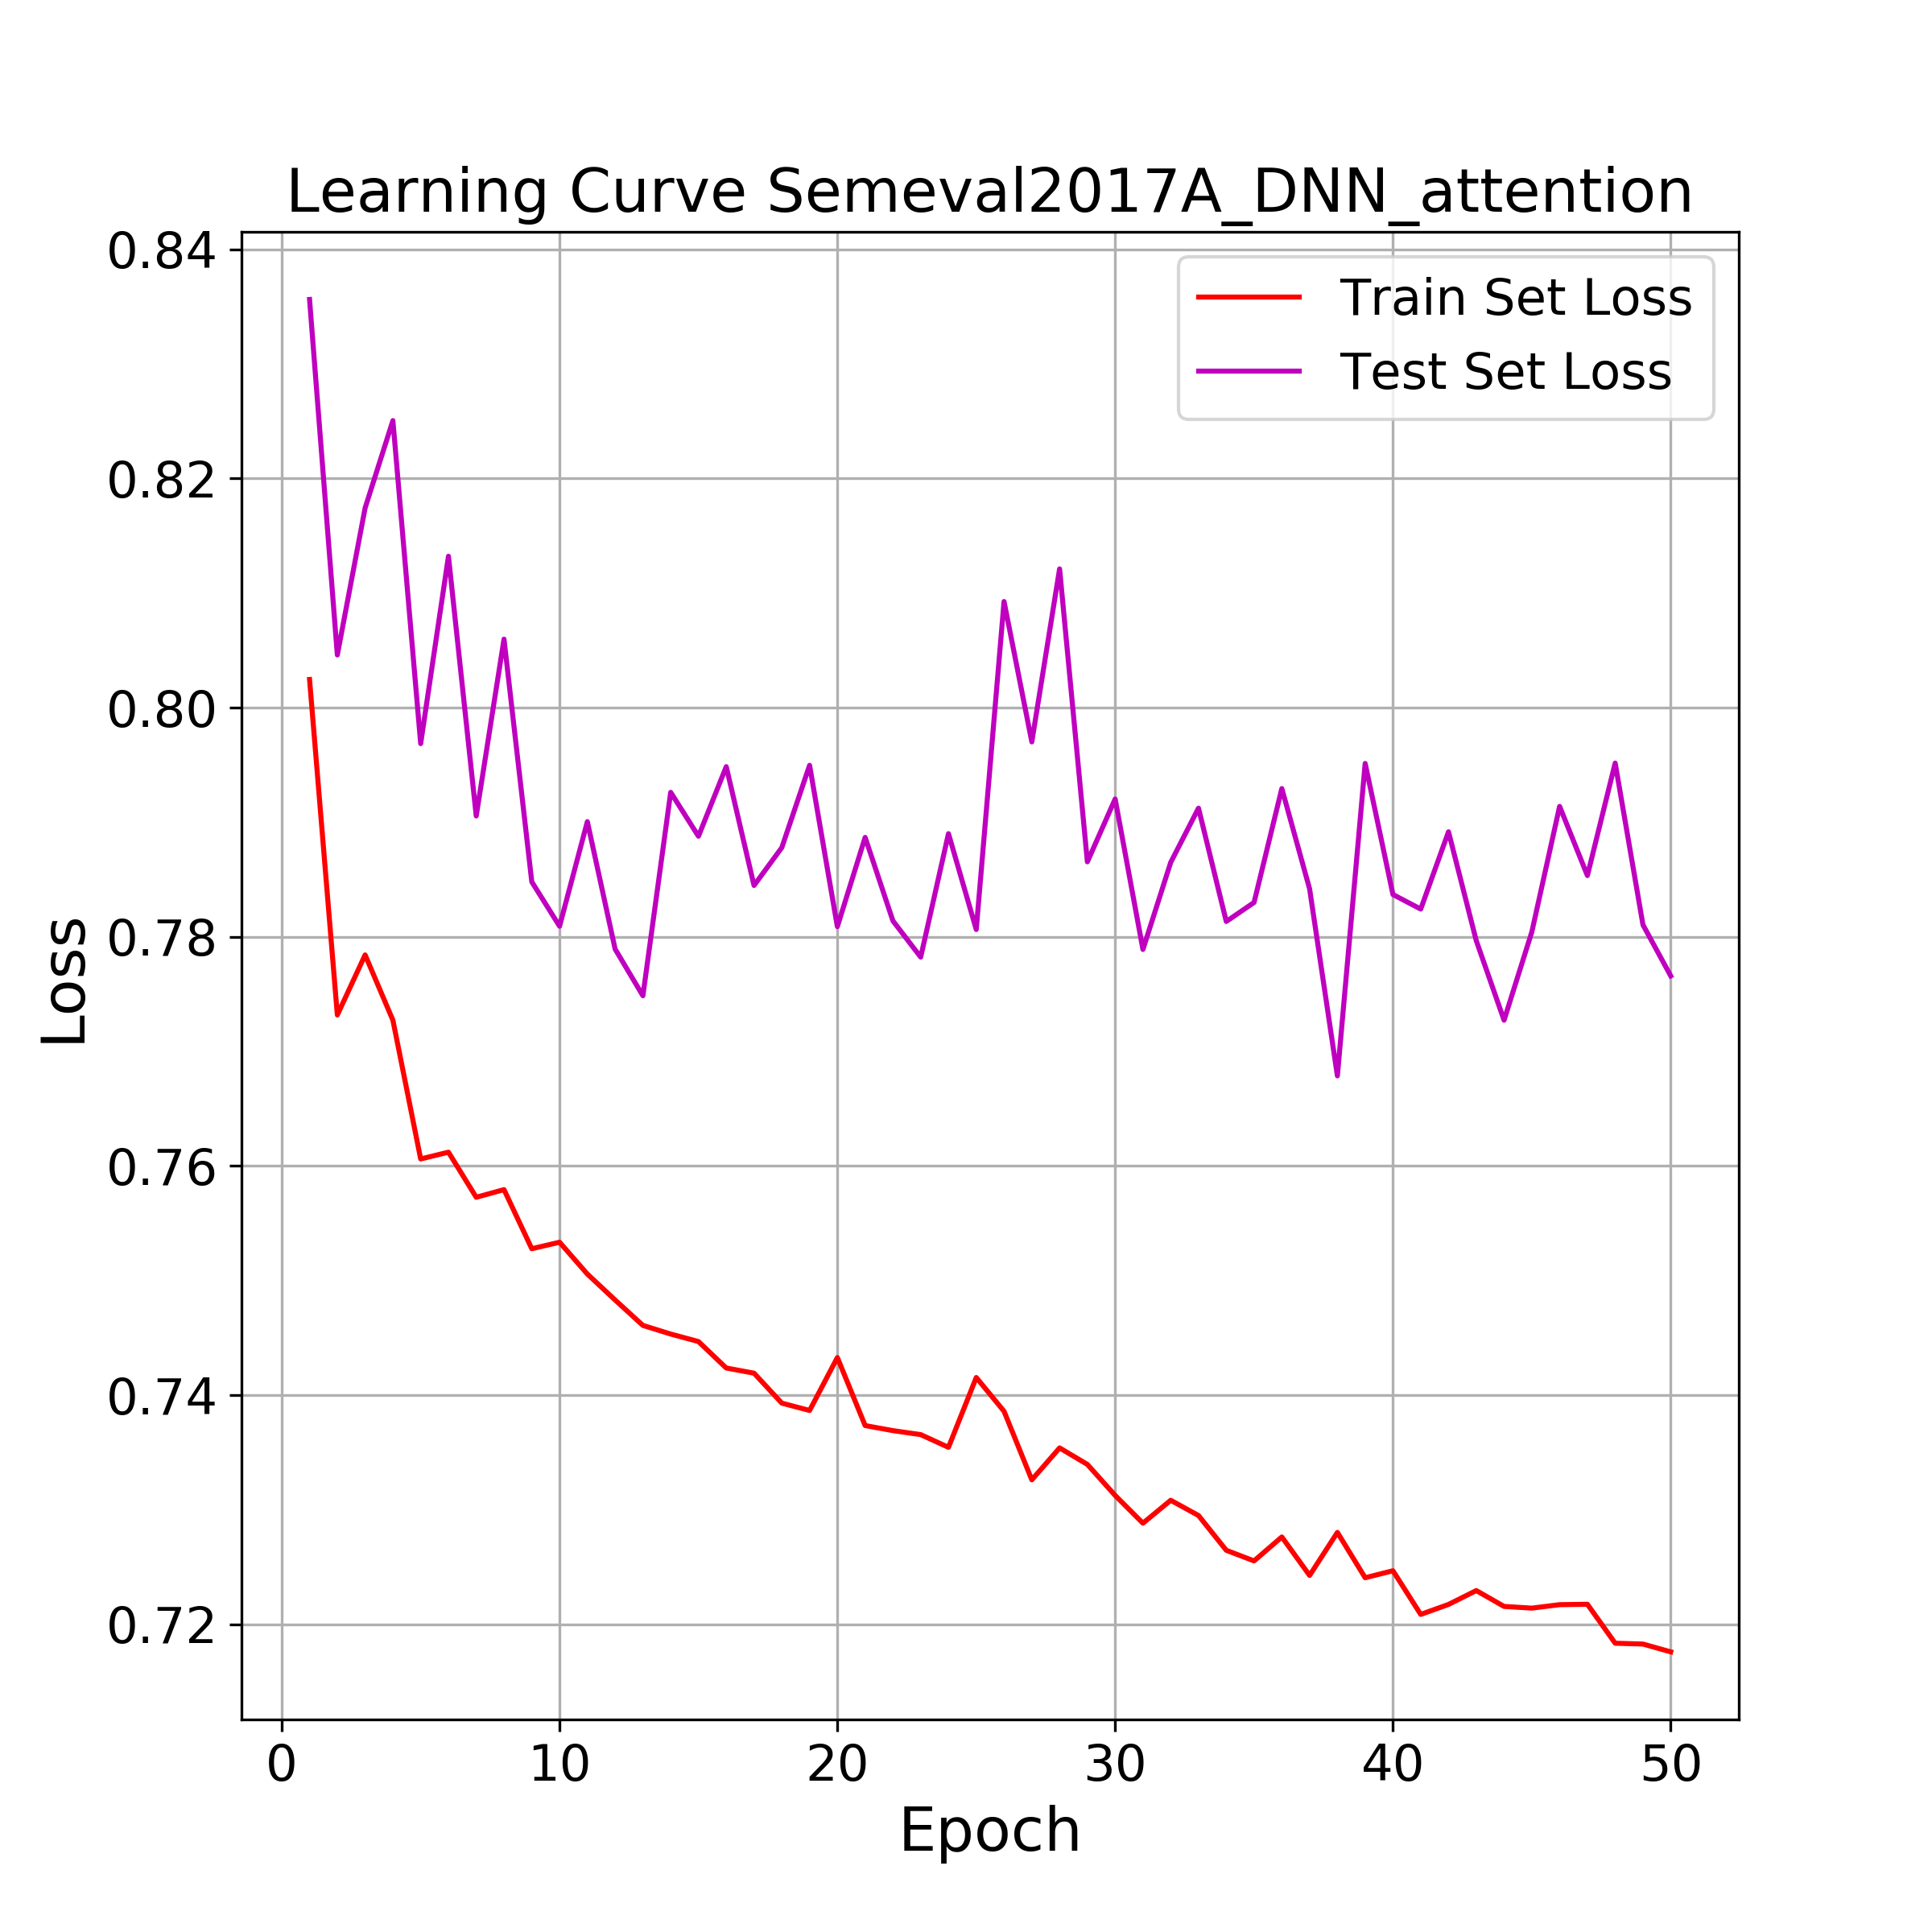
\includegraphics[width=0.6\linewidth]{./img/Semeval2017A/DNN_attention_loss}
	\caption{DNN with attention Learning Curve}
	\label{fig:sin}
\end{figure}


\begin{tabular}{lrrrr}
\toprule
DNN with attention &  precision &    recall &  f1-score &       support \\
\midrule
0            &   0.683162 &  0.569990 &  0.621466 &   3972.000000 \\
1            &   0.641534 &  0.746673 &  0.690122 &   5937.000000 \\
2            &   0.634466 &  0.550316 &  0.589402 &   2375.000000 \\
accuracy     &   0.651579 &  0.651579 &  0.651579 &      0.651579 \\
macro avg    &   0.653054 &  0.622326 &  0.633664 &  12284.000000 \\
weighted avg &   0.653628 &  0.651579 &  0.648449 &  12284.000000 \\
\bottomrule
\end{tabular}

Min Test Loss: 0.767867



\textbf{Ερώτημα 3.2:}
Αυτην την φορά εφαρμόζουμε attention στις εξόδους του LSTM. Και τα αποτελέσματα προκύπτουν:

\begin{figure}[h!]
	\centering
	\includegraphics[width=0.6\linewidth]{./img/Semeval2017A/lSTM_attention_loss}
	\caption{LSTM with attention Learning Curve}
	\label{fig:sin}
\end{figure}


\begin{tabular}{lrrrr}
\toprule
LSTM with attention &  precision &    recall &  f1-score &      support \\
\midrule
0            &   0.675668 &  0.592145 &  0.631155 &   3972.00000 \\
1            &   0.653687 &  0.718208 &  0.684430 &   5937.00000 \\
2            &   0.621491 &  0.596632 &  0.608808 &   2375.00000 \\
accuracy     &   0.653940 &  0.653940 &  0.653940 &      0.65394 \\
macro avg    &   0.650282 &  0.635661 &  0.641464 &  12284.00000 \\
weighted avg &   0.654570 &  0.653940 &  0.652583 &  12284.00000 \\
\bottomrule
\end{tabular}

Min Test Loss: 0.765446




\subsection{Ερώτημα 4}

Στο ερώτημα αυτό πειραματιζόμαστε με Bidirectional LSTM. Έχουμε χρησημοποιήσει στην υλοποίηση μας padded sequence, συνεπώς ο χειρισμός ακολουθιών μεταβλητού μήκους είναι εύκολος σε κάθε περίπτωση.

\textbf{Ερώτημα 4.1:}
Χρησιμοποιούμε bidirectional LSTM με mean, max pooling αναπαράσταση:

\begin{figure}[h!]
	\centering
	\includegraphics[width=0.6\linewidth]{./img/Semeval2017A/LSTM_pooling_Β_loss}
	\caption{LSTM pooling Bidirectional}
	\label{fig:sin}
\end{figure}


\begin{tabular}{lrrrr}
\toprule
LSTM pooling B &  precision &    recall &  f1-score &   support \\
\midrule
0            &   0.659361 &  0.628651 &  0.643640 &   3972.000000 \\
1            &   0.664191 &  0.692943 &  0.678262 &   5937.000000 \\
2            &   0.624403 &  0.605474 &  0.614793 &   2375.000000 \\
accuracy     &   0.655243 &  0.655243 &  0.655243 &      0.655243 \\
macro avg    &   0.649318 &  0.642356 &  0.645565 &  12284.000000 \\
weighted avg &   0.654937 &  0.655243 &  0.654796 &  12284.000000 \\
\bottomrule
\end{tabular}

Min Test Loss: 0.757021


\textbf{Ερώτημα 4.2:}
Χρησιμοποιούμε attention μηχανισμό και Bidirectional LSTM.

\begin{figure}[h]
	\centering
	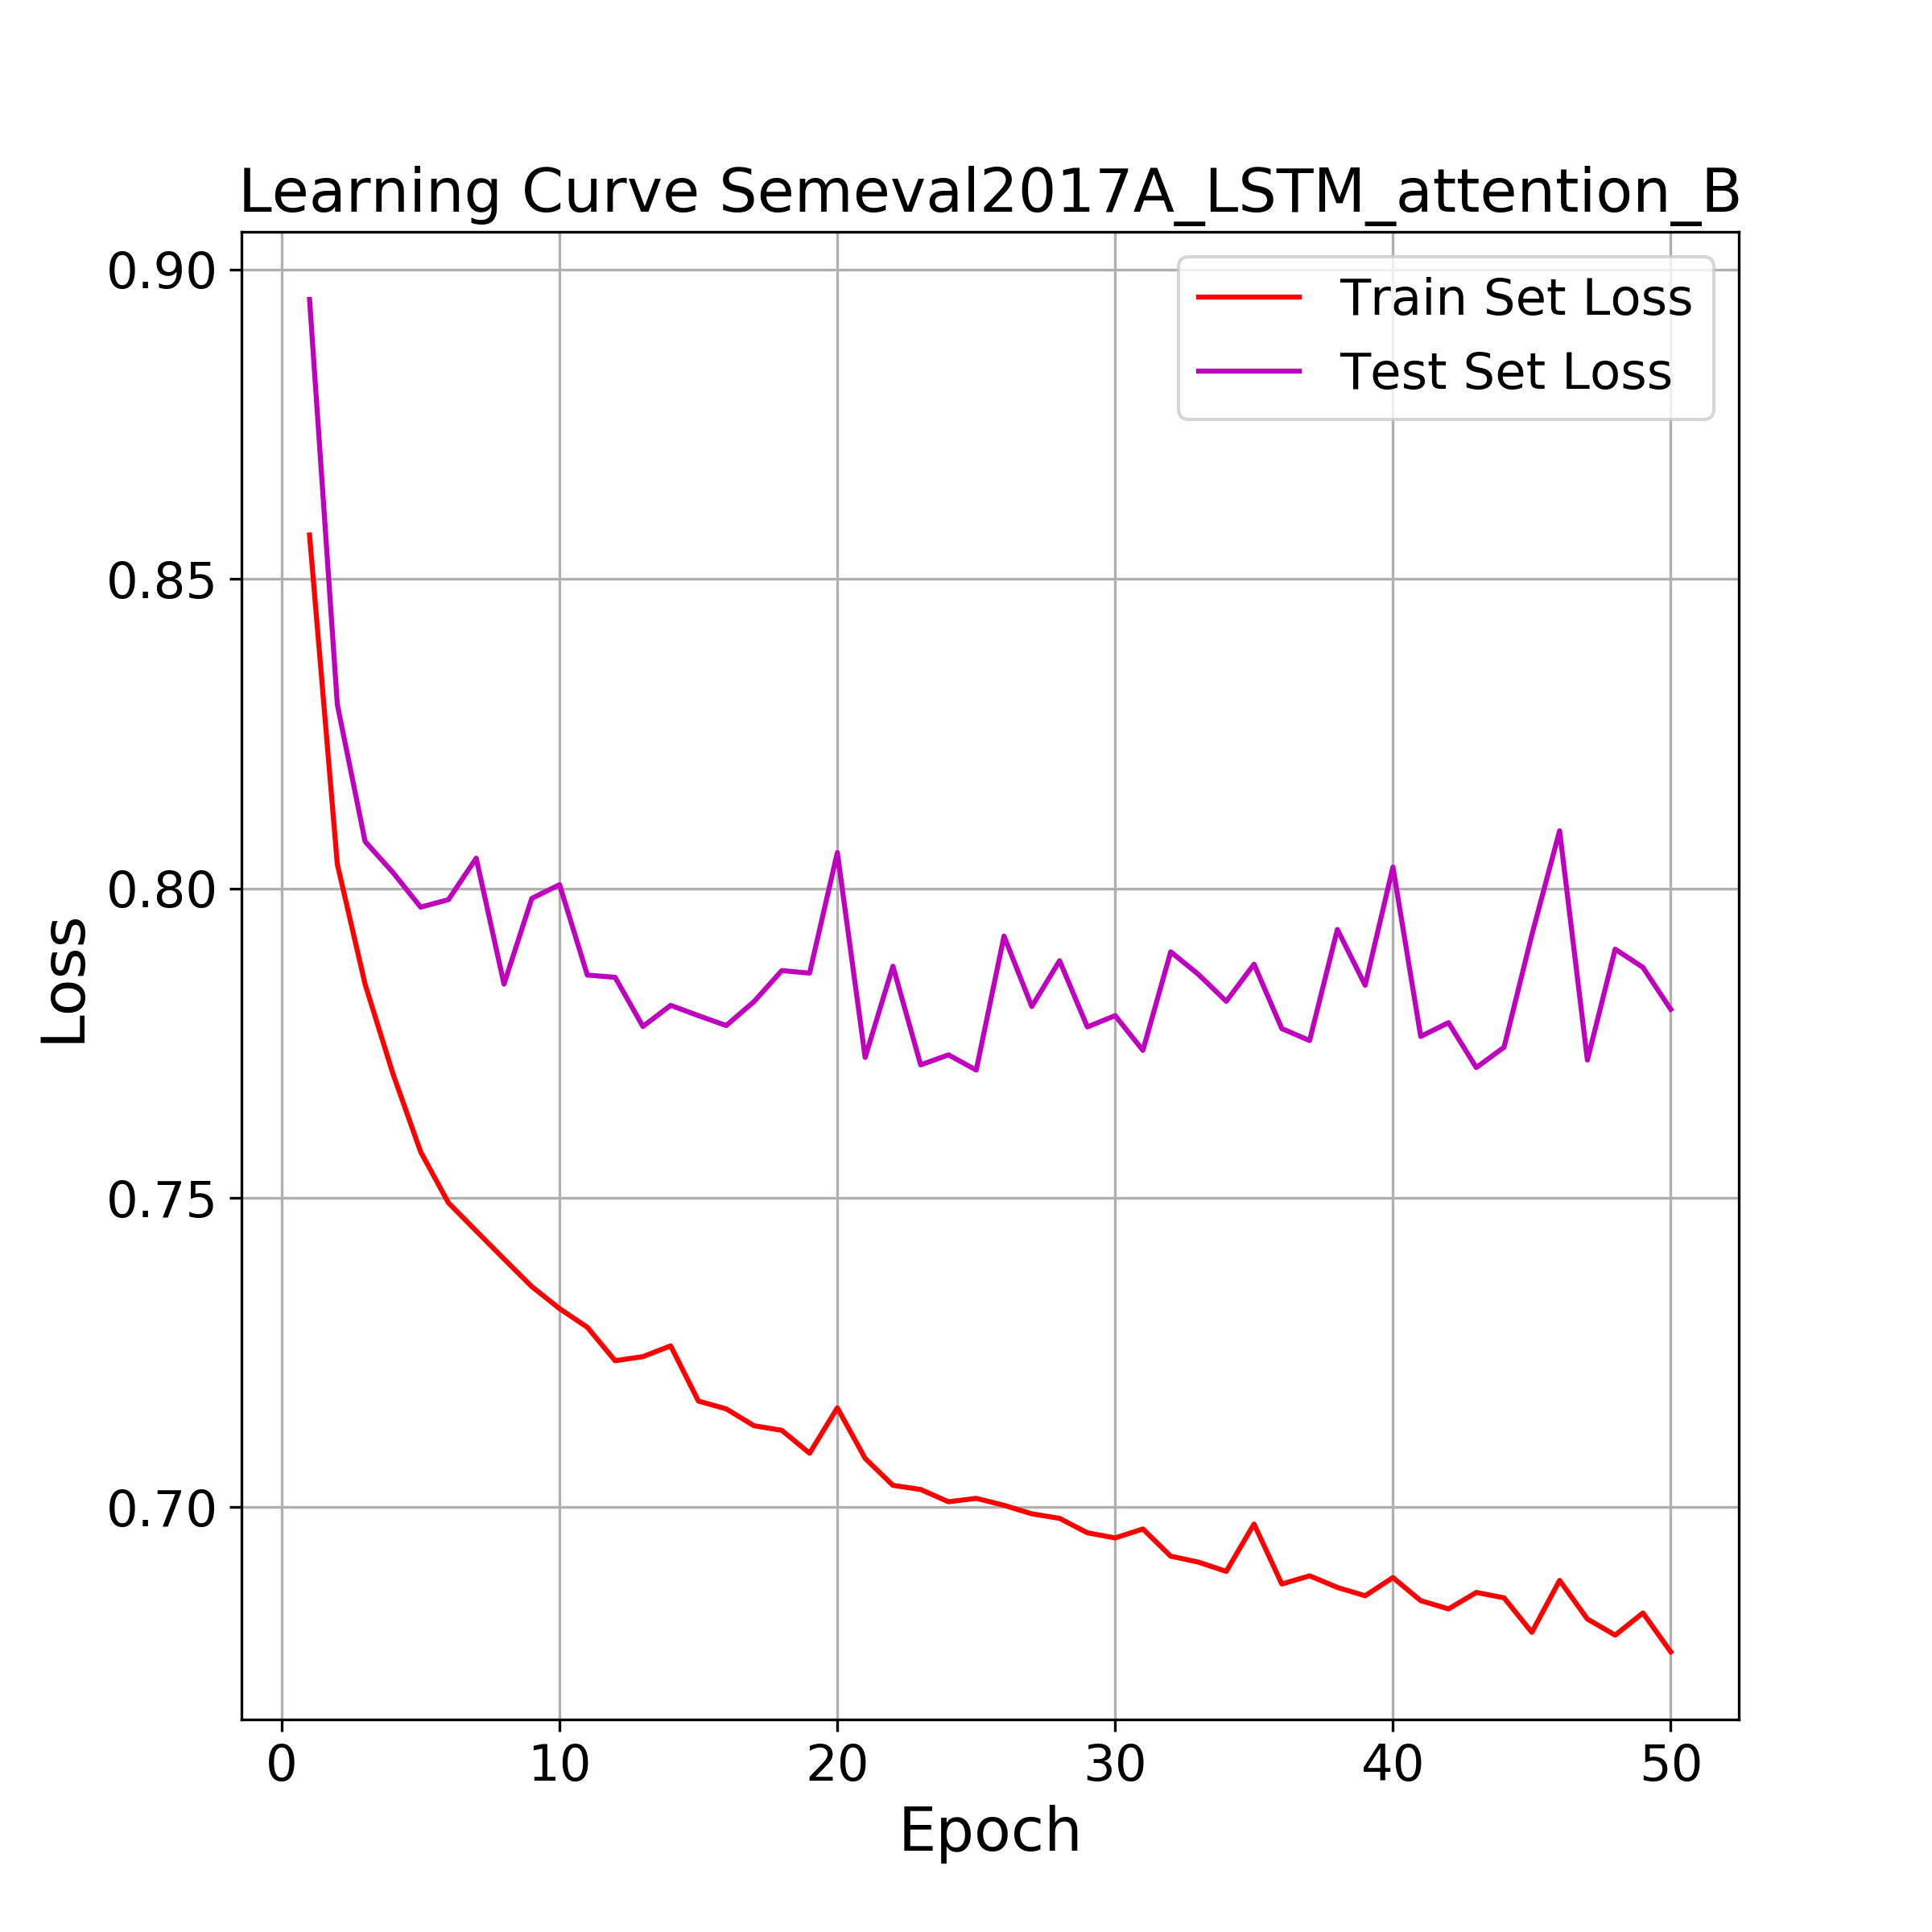
\includegraphics[width=0.6\linewidth]{./img/Semeval2017A/LSTM_attention_B_loss}
	\caption{LSTM attention Bidirectional}
	\label{fig:sin}
\end{figure}

\begin{tabular}{lrrrr}
\toprule
LSTM attention Bidirectional &  precision &    recall &  f1-score &       support \\
\midrule
0            &   0.677026 &  0.586858 &  0.628726 &   3972.000000 \\
1            &   0.652542 &  0.713323 &  0.681580 &   5937.000000 \\
2            &   0.614207 &  0.608000 &  0.611088 &   2375.000000 \\
accuracy     &   0.652068 &  0.652068 &  0.652068 &      0.652068 \\
macro avg    &   0.647925 &  0.636060 &  0.640465 &  12284.000000 \\
weighted avg &   0.653047 &  0.652068 &  0.650861 &  12284.000000 \\
\bottomrule
\end{tabular}

Min Test Loss: 0.770644


\subsection{Ερώτημα 5}
Το καλύτερο μοντέλο προκύπτει με ελαχιστη διαφορά το LSTM pooling bidirectional. Γενικά τα losses είναι αρκετά κοντά και δεν διακρίνουμε μεγάλες διαφορές στο accuracy. Παρατηρούμε ότι τα LSTM έχουν αρκετά μικρότερο training loss απο ότι τα DNN, χωρίς όμως σημαντική βελτίωση στην ακρίβεια. Αυτό συμβαίνει γιατί όπως φαίνεται και απο τα learning curves το generalization error είναι τεράστιο. θα πρέπει λοιπόν να αξιοποιήσουμε τεχνικές regualrization για να δούμε μέχρι που μπορεί αληθινά να φτάσει η απόδοση των LSTM στο test set.

Αποθηκέυουμε τις προβλέψεις σε .txt αρχείο που επισυνάπτεται.  



\textbf{Ερώτημα 5.2:}

Στον παρακάτω πίνακα φαίνεται το Minimum Test Loss των μοντέλων στα οποία έχουμε χρησιμοποιήσει attention weights:

\begin{center}
\begin{tabular}{ |c|c|c|c| } 
 \hline
    &DNN & LSTM & LSTM Bidirectional \\
 \hline 
 Loss & 0.767867 & 0.765446 & 0.770644\\
  \hline 
\end{tabular}
\end{center}

Άρα επιλέγουμε το LSTM μοντέλο για το οποίο κάνουμε visualize τα αποτελέσματα του με τη βοήθεια του NeAt-Vision (https://github.com/cbaziotis/neat-vision) . Για να το χρησιμοποιήσουμε φτιάξαμε δύο αρχεία .json ένα με τα labels και ένα για την αντιστοίχιση του κειμένου με τα attention weights καθώς και το prediction.  

Παρακάτω βλέπουμε κάποια tweets τα οποία κατατάσσονται στη σωστή κατηγορία και φαίνεται πως στις λέξεις έχουν δοθεί βάρη τα οποία δικαιολογούν τη σωστή κατάταξη του tweet.

Positive tweet:
\begin{figure}[h]
	\centering
		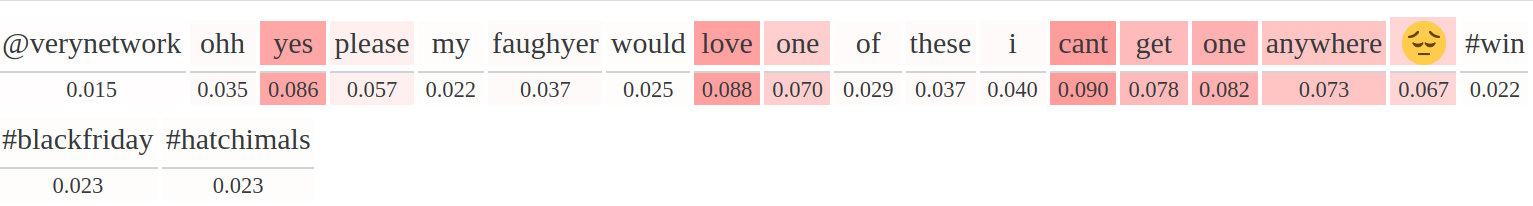
\includegraphics[width=0.9\linewidth]{480}
	\label{fig:sin}
\end{figure}

Negative tweet:
\begin{figure}[h]
	\centering
		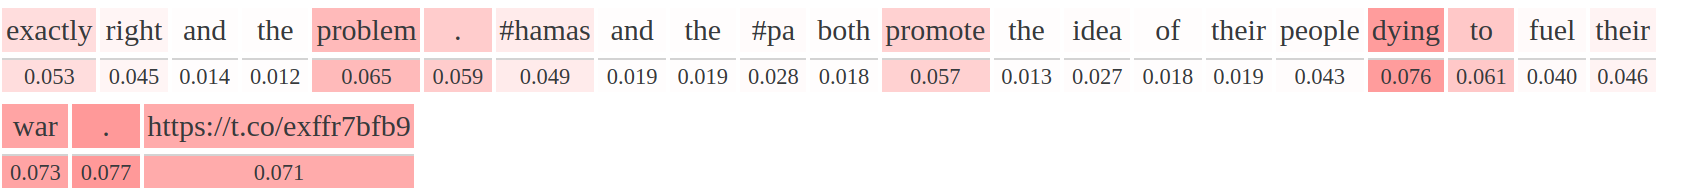
\includegraphics[width=0.9\linewidth]{321}
	\label{fig:sin}
\end{figure}

Neutral tweet:

\begin{figure}[h]
	\centering
		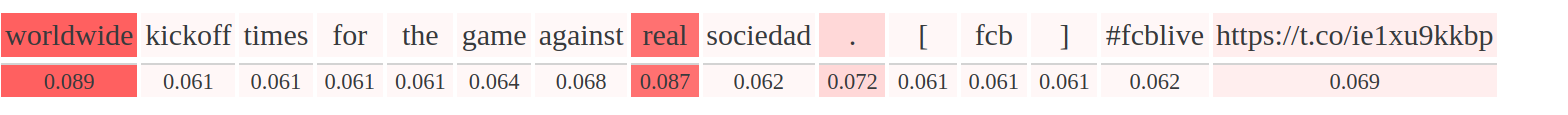
\includegraphics[width=0.9\linewidth]{162}
	\label{fig:sin}
\end{figure}

Σε όλα αυτά τα tweets βλέπουμε ότι δίνεται attention σε λέξεις που έχουν θετικό, αρνητικό και ουδέτερο νόημα αντίσοιχα. 

Υπάρχουν όμως και κάποια tweets που δεν κατατάσσονται σωστά. Τα tweets αυτά είναι κυρίως neutral στα οποία δίνεται η κατηγορία positive ή negative λόγω κάποιων "θετικών" ή "αρνητικών" λέξεων στις οποίες έχουν δοθεί μεγαλύτερα βάρη. Μερικά παραδείγματα είναι τα εξής:

Label: neutral -- Prediction: negative

\begin{figure}[h]
	\centering
		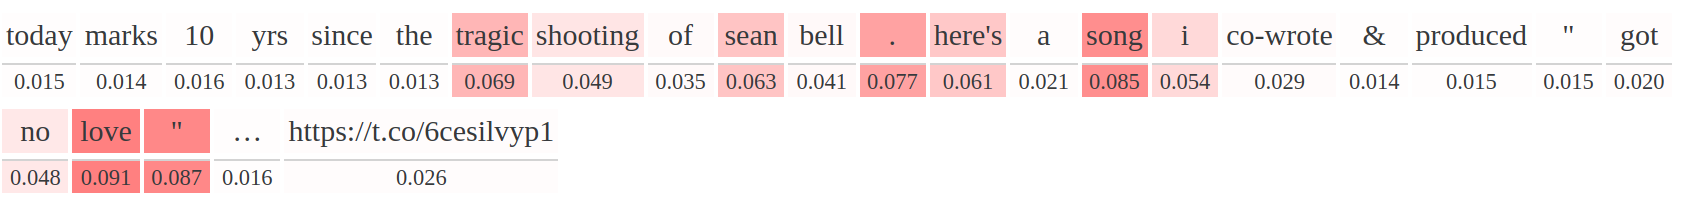
\includegraphics[width=0.9\linewidth]{100}
	\label{fig:sin}
\end{figure}


Σε αυτό το sample βλεπουμε ότι έχει δοθεί attention σε πολλές αρνητικές λέξεις και για αυτό καταττάσεται σε negative.

Label: neutral -- Prediction: positive

\begin{figure}[h]
	\centering
		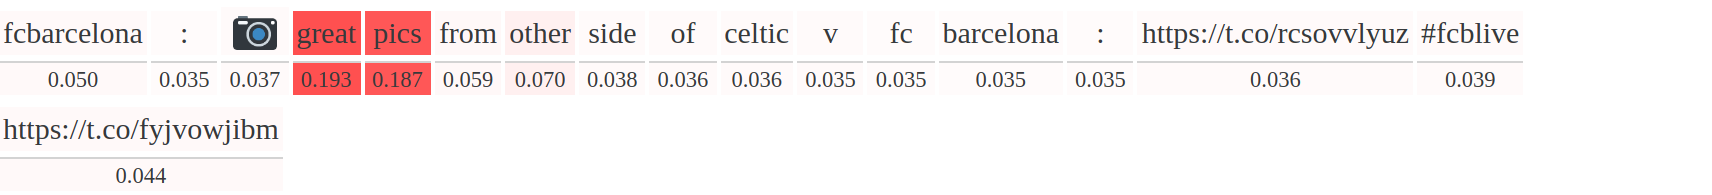
\includegraphics[width=0.9\linewidth]{123}
	\label{fig:sin}
\end{figure}


Αντίστοιχα σε αυτό το tweet βλέπουμε ότι στις λέξεις great pics έχουμε μεγάλα attention βάρη αλλά στο σύνολο της η πρόταση είναι ουδέτερη και όχι θετική όπως συμπεραίνεται με βάση αυτές τις δύο λέξεις. 

Τέλος, σπάνια ένα αρνητικό tweet κατατάσσεται σε θετικό και αντίστροφα. Αυτό γίνεται στις περιπτώσεις που το tweet κάποιο αρνητικό tweet περιέχει λέξεις με θετικό νόημα ή οποίες μπορεί να είναι ειρωνικές πχ και αντίστροφα. Αυτό συμβαίνει και στο παρακάτω παράδειγμα.

\begin{figure}[h!]
	\centering
		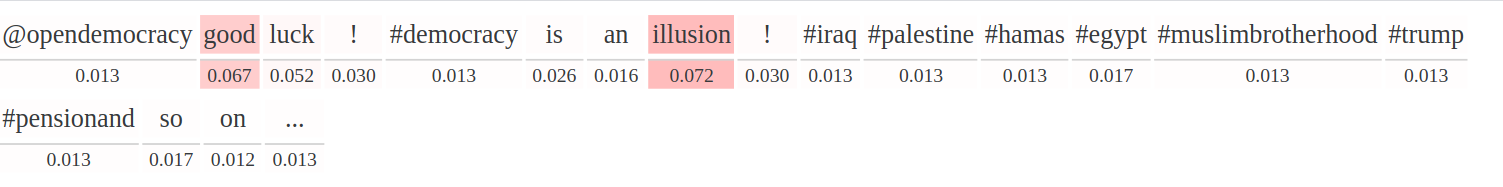
\includegraphics[width=0.9\linewidth]{382}
	\label{fig:sin}
\end{figure}

\pagebreak
Παρατηρούμε ότι το συγκεκριμένο tweet είναι negative αλλά το prediction μας λέει ότι είναι positive. Αυτό συμβαίνει γιατί όπως βλέπουμε το attention δίνει βάρος στις λέξεις good luck ! και illusion αντί να κοιτάξει όλο το context για να δει ότι έχει έναν αρνητικό τόνο ειρωνίας. 

\textbf{Ερώτημα 5.3:}

Σε αυτό το ερώτημα θα συγκρίνουμε το DNN με τη χρήση του μηχανισμού attention με το αντίστοιχο LSTM μονέλο με attention. 
Παρατηρούμε ότι το LSTM κατανέμει με διαφορετικό τρόπο τα βάρη στις λέξεις των tweets. Αυτό συμβαίνει γιατί για κάθε λέξη έχει κρατήσει πληροφορία για τις προηγούμενες λέξεις από αυτή. Αντίθετα, το DNN κοιτάει κάθε λέξη ξεχωριστά και όχι το νοήμα που μπορεί να έχει στην πρόταση και έτσι δεν φαίνεται να δίνει καλά attention weights στα tweets. 

Παρακάτω φαίνονται 3 αποτελέσματα από τις κατανομές των attention weights του DNN και για τα ίδια παραδείγματα του LSTM.

\begin{figure}[h!]
	\centering
		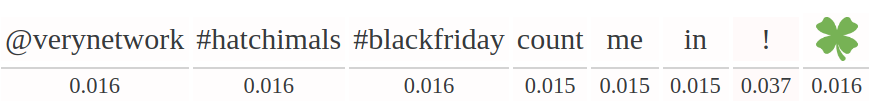
\includegraphics[width=0.9\linewidth]{473_DNN.png}
	\label{fig:sin}
\end{figure}
\begin{figure}[h!]
	\centering
		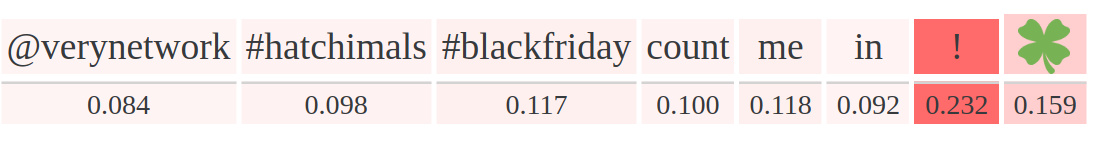
\includegraphics[width=0.9\linewidth]{473_LSTM.png}
	\label{fig:sin}
\end{figure}

Παρατηρούμε ότι στο DNN δεν έχει δωθεί σημαντικό βάρος σε καμία από τις λέξεις του κειμένου και το tweet δεν κατατάσσεται στη σωστή κατηγορία. Αντίθετα, στο LSTM βλέπουμε ότι δίνεται βάρος στο θαυμαστικό και στο τριφύλλι και με βάση αυτά κατατάσσεται στη σωστή κατηγορία.  

\begin{figure}[h!]
	\centering
		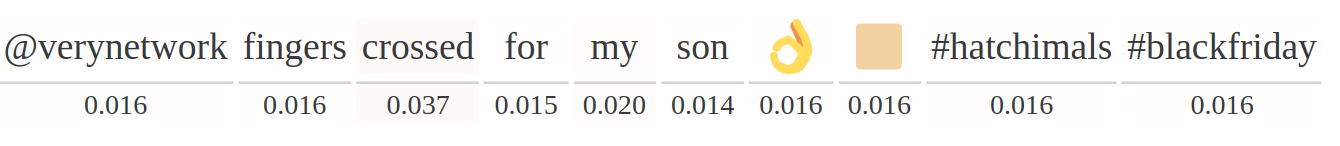
\includegraphics[width=0.9\linewidth]{500_DNN.png}
	\label{fig:sin}
\end{figure}
\begin{figure}[h!]
	\centering
		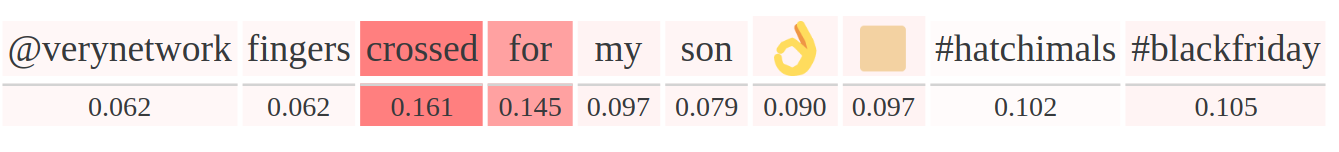
\includegraphics[width=0.9\linewidth]{500_LSTM.png}
	\label{fig:sin}
\end{figure}


Σε αυτό το παράδειγμα βλέπουμε ότι το DNN έκανε τη σωστή πρόβλεψη σε αντίθεση με το LSTM. Αυτό συμβαίνει γιατί το LSTM δίνει βάρος στις λέξεις crossed for σε αντίθεση με το DNN που δεν δίνει υψηλό βάρος σε καμία λέξη και άρα καταττάσει σωστά το tweet.

\begin{figure}[h!]
	\centering
		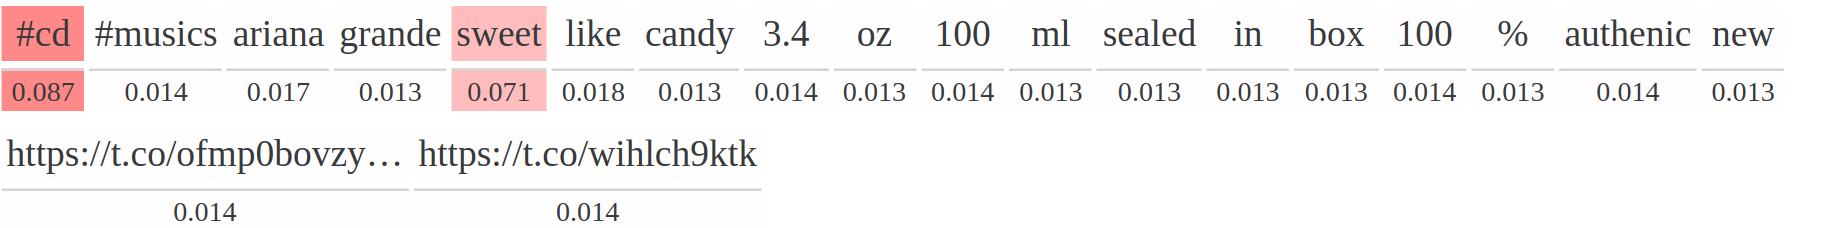
\includegraphics[width=0.9\linewidth]{3_DNN.png}
	\label{fig:sin}
\end{figure}
\begin{figure}[h!]
	\centering
		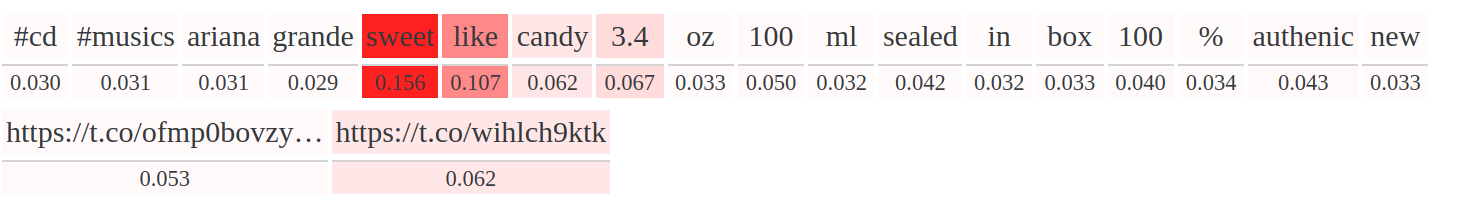
\includegraphics[width=0.9\linewidth]{3_LSTM.png}
	\label{fig:sin}
\end{figure}


Σε αυτή την περίπτωση βλέπουμε ότι και τα δύο μοντέλα έχουν κάνει σωστή πρόβλεψη αλλά έχουμε attention weights σε διαφορετικές λέξεις.
Παρατηρούμε επίσης ότι το LSTM έδωσε πολύ μεγάλο βάρος στη λέξη sweet σε αντίθεση με το DNN. 

Διαισθητικά αυτο που περιμένουμε απο την σύγκριση είναι οτι το DNN θα δίνει σημασία σε μεμονομένες συγκινησιακά φορτισμένες λέξεις αφού δεν έχει πληροφορία συμφράζομενων. Το LSTM θα μπορεί να επιλέξει σωστότερα σημαντικές λέξεις με βάση το περιεχόμενο όλου του κειμένου, πράγμα που το οδηγεί σε καλύτερες προβλέψεις.

Καταλήγουμε στο συμπέρασμα ότι ο μηχανισμός attention λειτουργεί καλύτερα με LSTM καθώς το DNN τείνει σε ομοιόμορφες κατανομές, που δεν μας είναι στην πράξη ιδιαίτερα χρήσιμες.

Σημείωση: Τα labels στα παραπάνω παραδείγματα λείπουν λόγω bug τελευταίας στιγμής με το NeΑt-vision, οι παρατηρήσεις όμως αντιστοιχούν στα αληθινά labels που προβλέπει το μοντέλο μας.


\subsection{Ερώτημα 6}
\textbf{Ερώτημα 6.1:}
Επιλέγουμε να εισάγουμε BoW αναπαράσταση με χρήση tf-idf σε όλο το corpus τα οποία υπολογίζονται στην dataloading.py. Το tf-idf είναι βάρος για κάθε λέξη για κάθε sample (document) πάνω στα word embeddings, και έτσι υπολογίζουμε την ενδιάμεση αναπαράσταση και μετά μπορούμε να εφαρμόσουμε οποιαδήποτε απο τις παραπάνω τεχνικές που αναφέραμε (LSTM,pooling,attention,...).

Εκπαιδέυσαμε μοντέλο LSTM με attention και tf-idf παρουσιάζουμε τα αποτελέσματα:


\begin{figure}[h!]
	\centering
	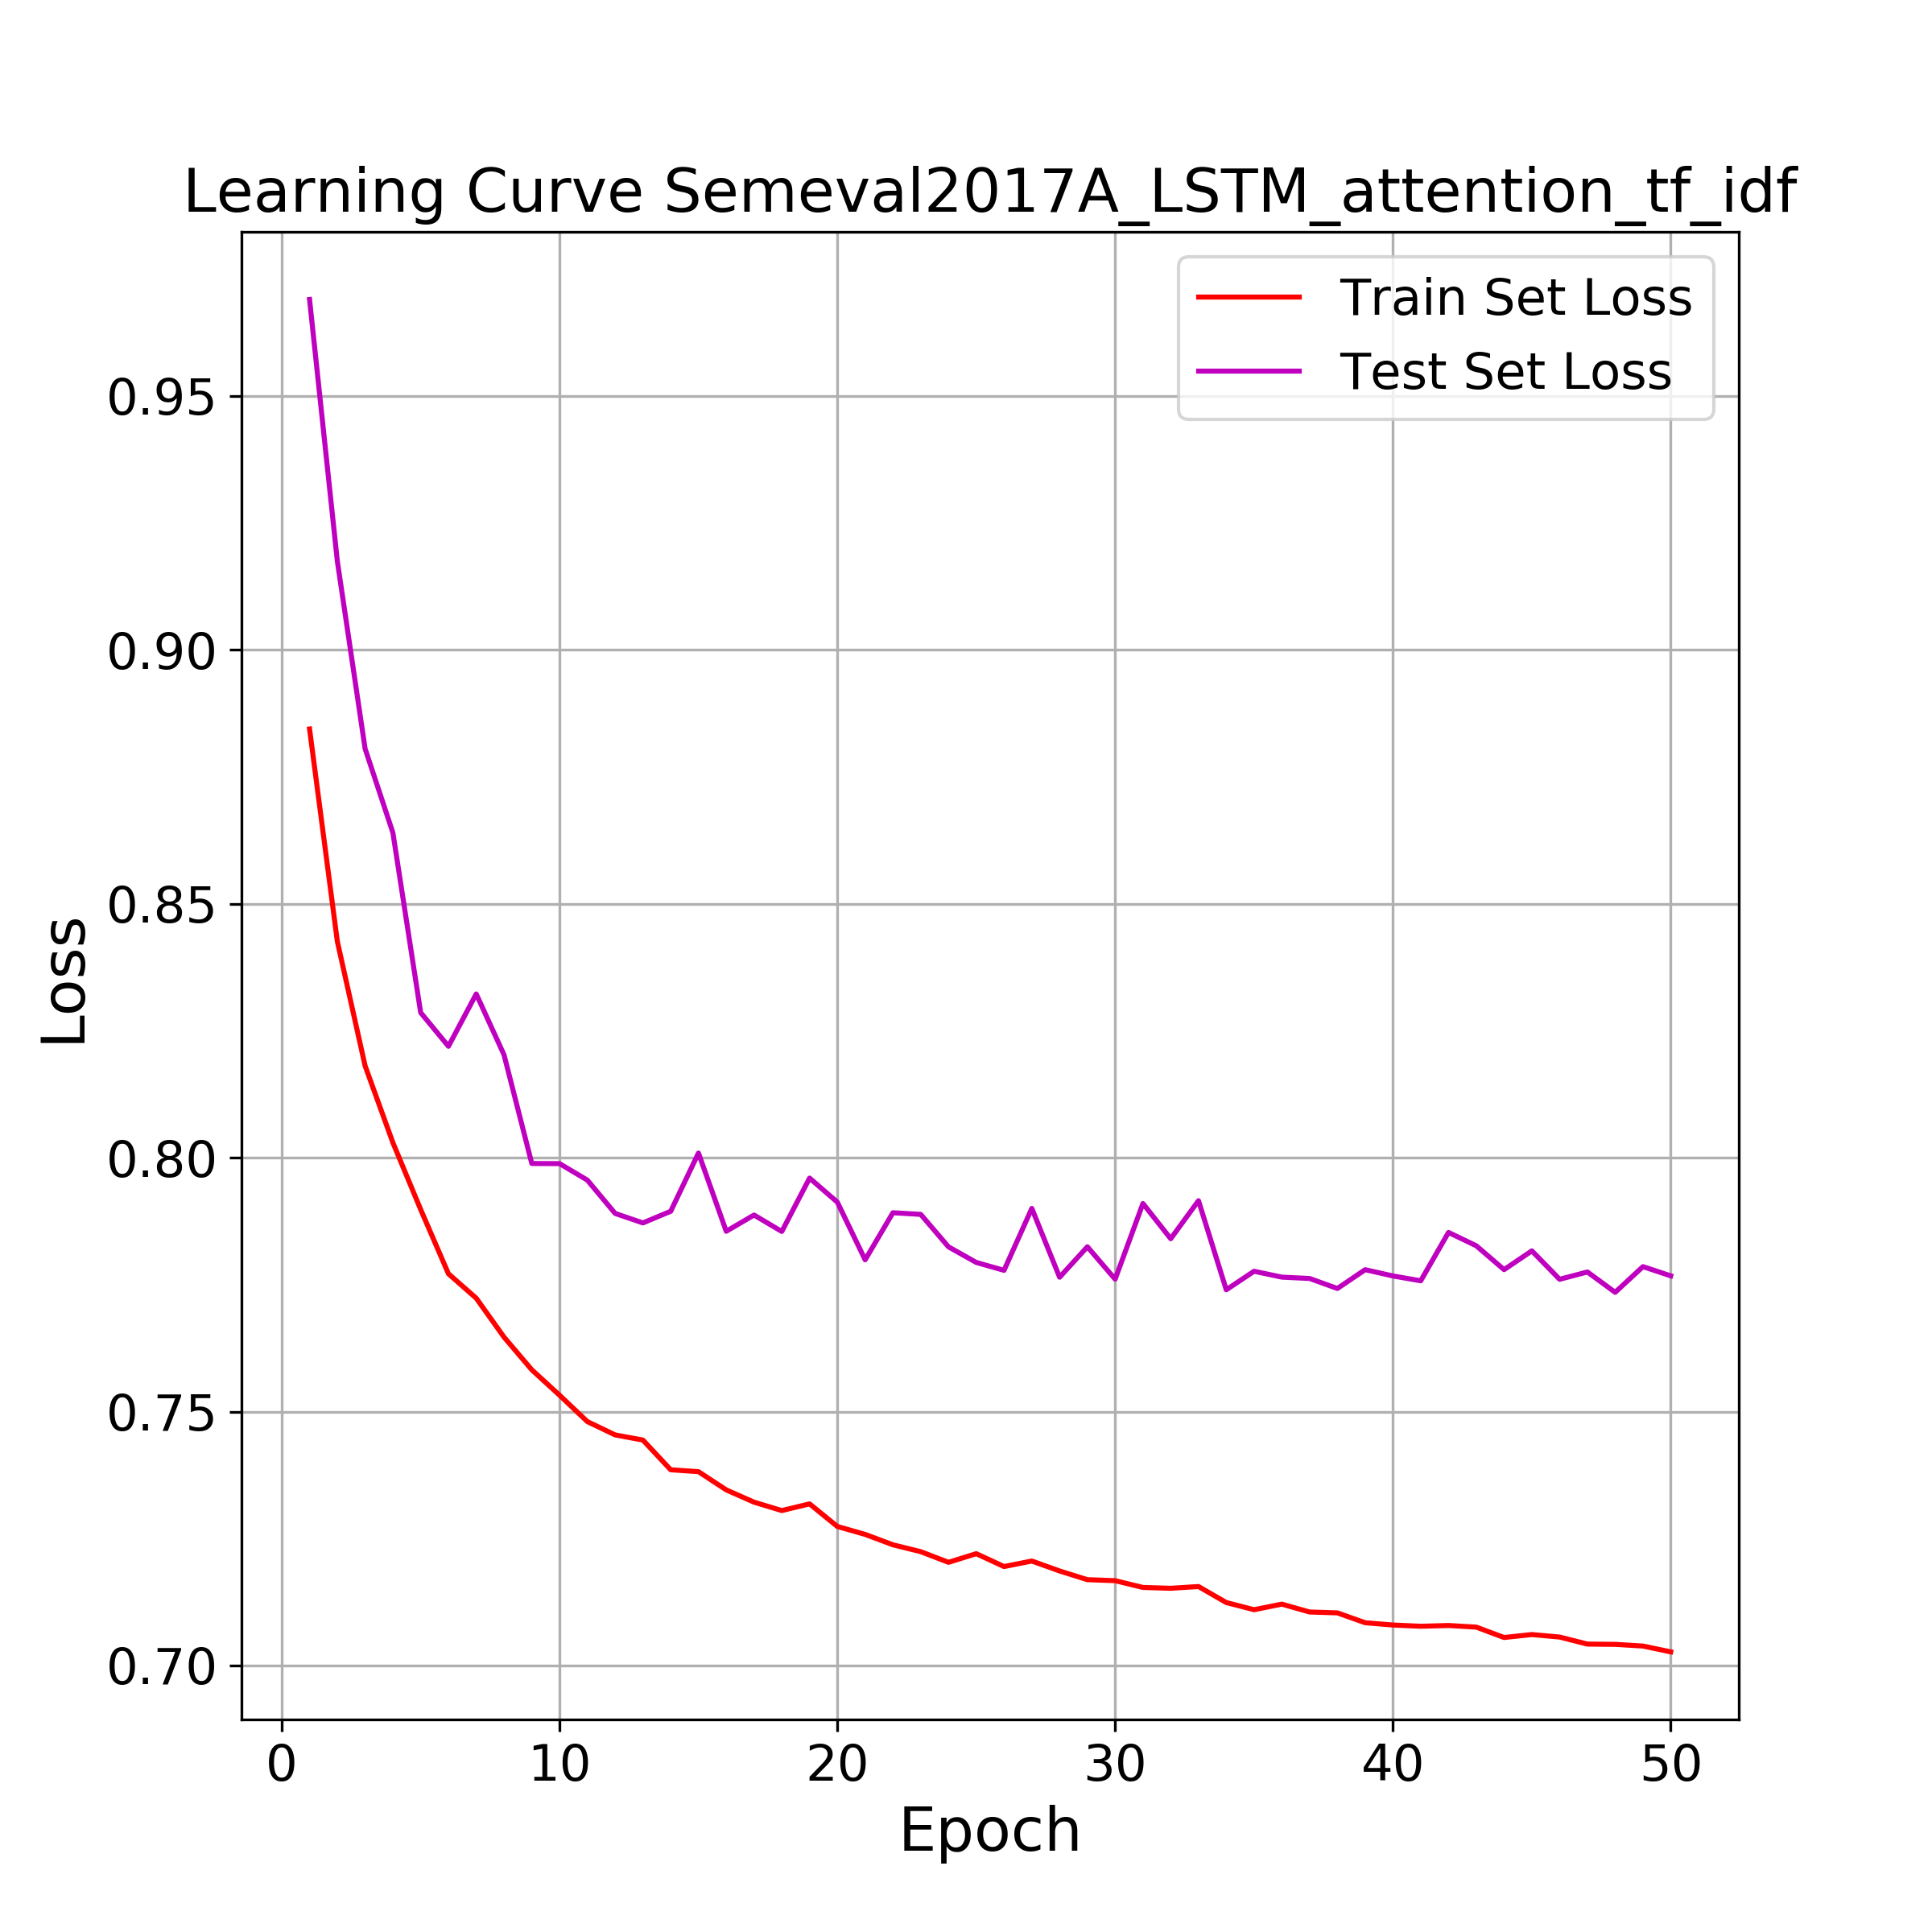
\includegraphics[width=0.6\linewidth]{./img/Semeval2017A/LSTM_attention_tf_idf_loss}
	\caption{LSTM attention tf-idf}
	\label{fig:sin}
\end{figure}

\begin{tabular}{lrrrr}
\toprule
{} &  precision &    recall &  f1-score &       support \\
\midrule
0            &   0.678826 &  0.576284 &  0.623366 &   3972.000000 \\
1            &   0.647068 &  0.709955 &  0.677054 &   5937.000000 \\
2            &   0.592577 &  0.598316 &  0.595433 &   2375.000000 \\
accuracy     &   0.645148 &  0.645148 &  0.645148 &      0.645148 \\
macro avg    &   0.639490 &  0.628185 &  0.631951 &  12284.000000 \\
weighted avg &   0.646801 &  0.645148 &  0.643913 &  12284.000000 \\
\bottomrule
\end{tabular}

Min Test Loss: 0.773480

Δεν παρατηρούμε βελτίωση

\textbf{Ερώτημα 6.2:}

Η αναπαράσταση BoW μετράει την συχνότητα εμφάνισης κάθε λέξης στα κείμενα που εξετάζουμε, στην περίπτωση της άσκησης την εμφάνιση της κάθε λέξης στα tweets. Αντίθετα, τα word embeddings για κάθε λέξη έχουν ένα vector, και για κάθε tweet μπορούμε να πάρουμε το μέσο όρο των embeddings κάθε λέξης. Άρα καταλαβαίνουμε ότι η μέση τιμή των word enbeddings βοηθάει στην κατανόηση του περιεχόμενου του κειμένου (tweet), ενώ αντίθετα η BoW αναπαράσταση μπορεί να βοηθήσει να γίνει classify ένα κείμενο (tweet) στο σύνολο του, δηλαδή σε σχέση με τα υπόλοιπα κείμενα (tweets). Αυτό συμβαίνει γιατί με τις BoW αναπαραστάσεις μπορούμε να δούμε ποιες λέξεις εμφανίζονται συχνά σε πολλά κείμενα και με αυτό τον τρόπο να τα ομαδοποιήσουμε. Άρα, στην συγκεκριμένη άσκηση θα μπορούσαμε να χρησιμοποιήσουμε την BoW αναπαράσταση για να χωρίσουμε τα tweets σε 3 κατηγορίες χωρίς να ξέρουμε το label τους και στη συνέχεια να δούμε πόσο καλά έγινε ο διαχωρσιμός αφού έχουμε τα labels των tweets.



\subsection{Ερώτημα 7}
Εφαρμόζουμε μεταφορά γνώσης για να βελτιώσουμε τις επιδόσεις ενός μοντέλου για τον υπολογισμό έντασης συναισθήματος. Ως source dataset χρησιμοποιήσαμε το 
Semeval 2017 Task4-A και ως target το SemEval-2018 Task 1: Affect in Tweets 6. Συμβουλευτήκαμε την σχετική βιβλιογραφία [Rosenthal et al., 2017], [Baziotis et al., 2018].

Για κάθε ένα απο τα συναισθήματα \{joy,fear,anger,sadness\} εκτελέσαμε μεταφορά γνώσης και παρουσιάζουμε τα αποτελέσματα:


Ενδιαφέρον είναι ότι σε μερικά συναισθήματα το test loss ξεκινάει χαμηλότερα απο το train loss, κάτι που οφείλεται φυσικά στην μεταφορά γνώσης. Υπολογίσαμε και τον Pearson corellation coefficient μιας και αυτή αυτή ειναι η βασική μετρική του αντίστοιχου Semeval task.


\begin{figure}[h!]
	\centering
	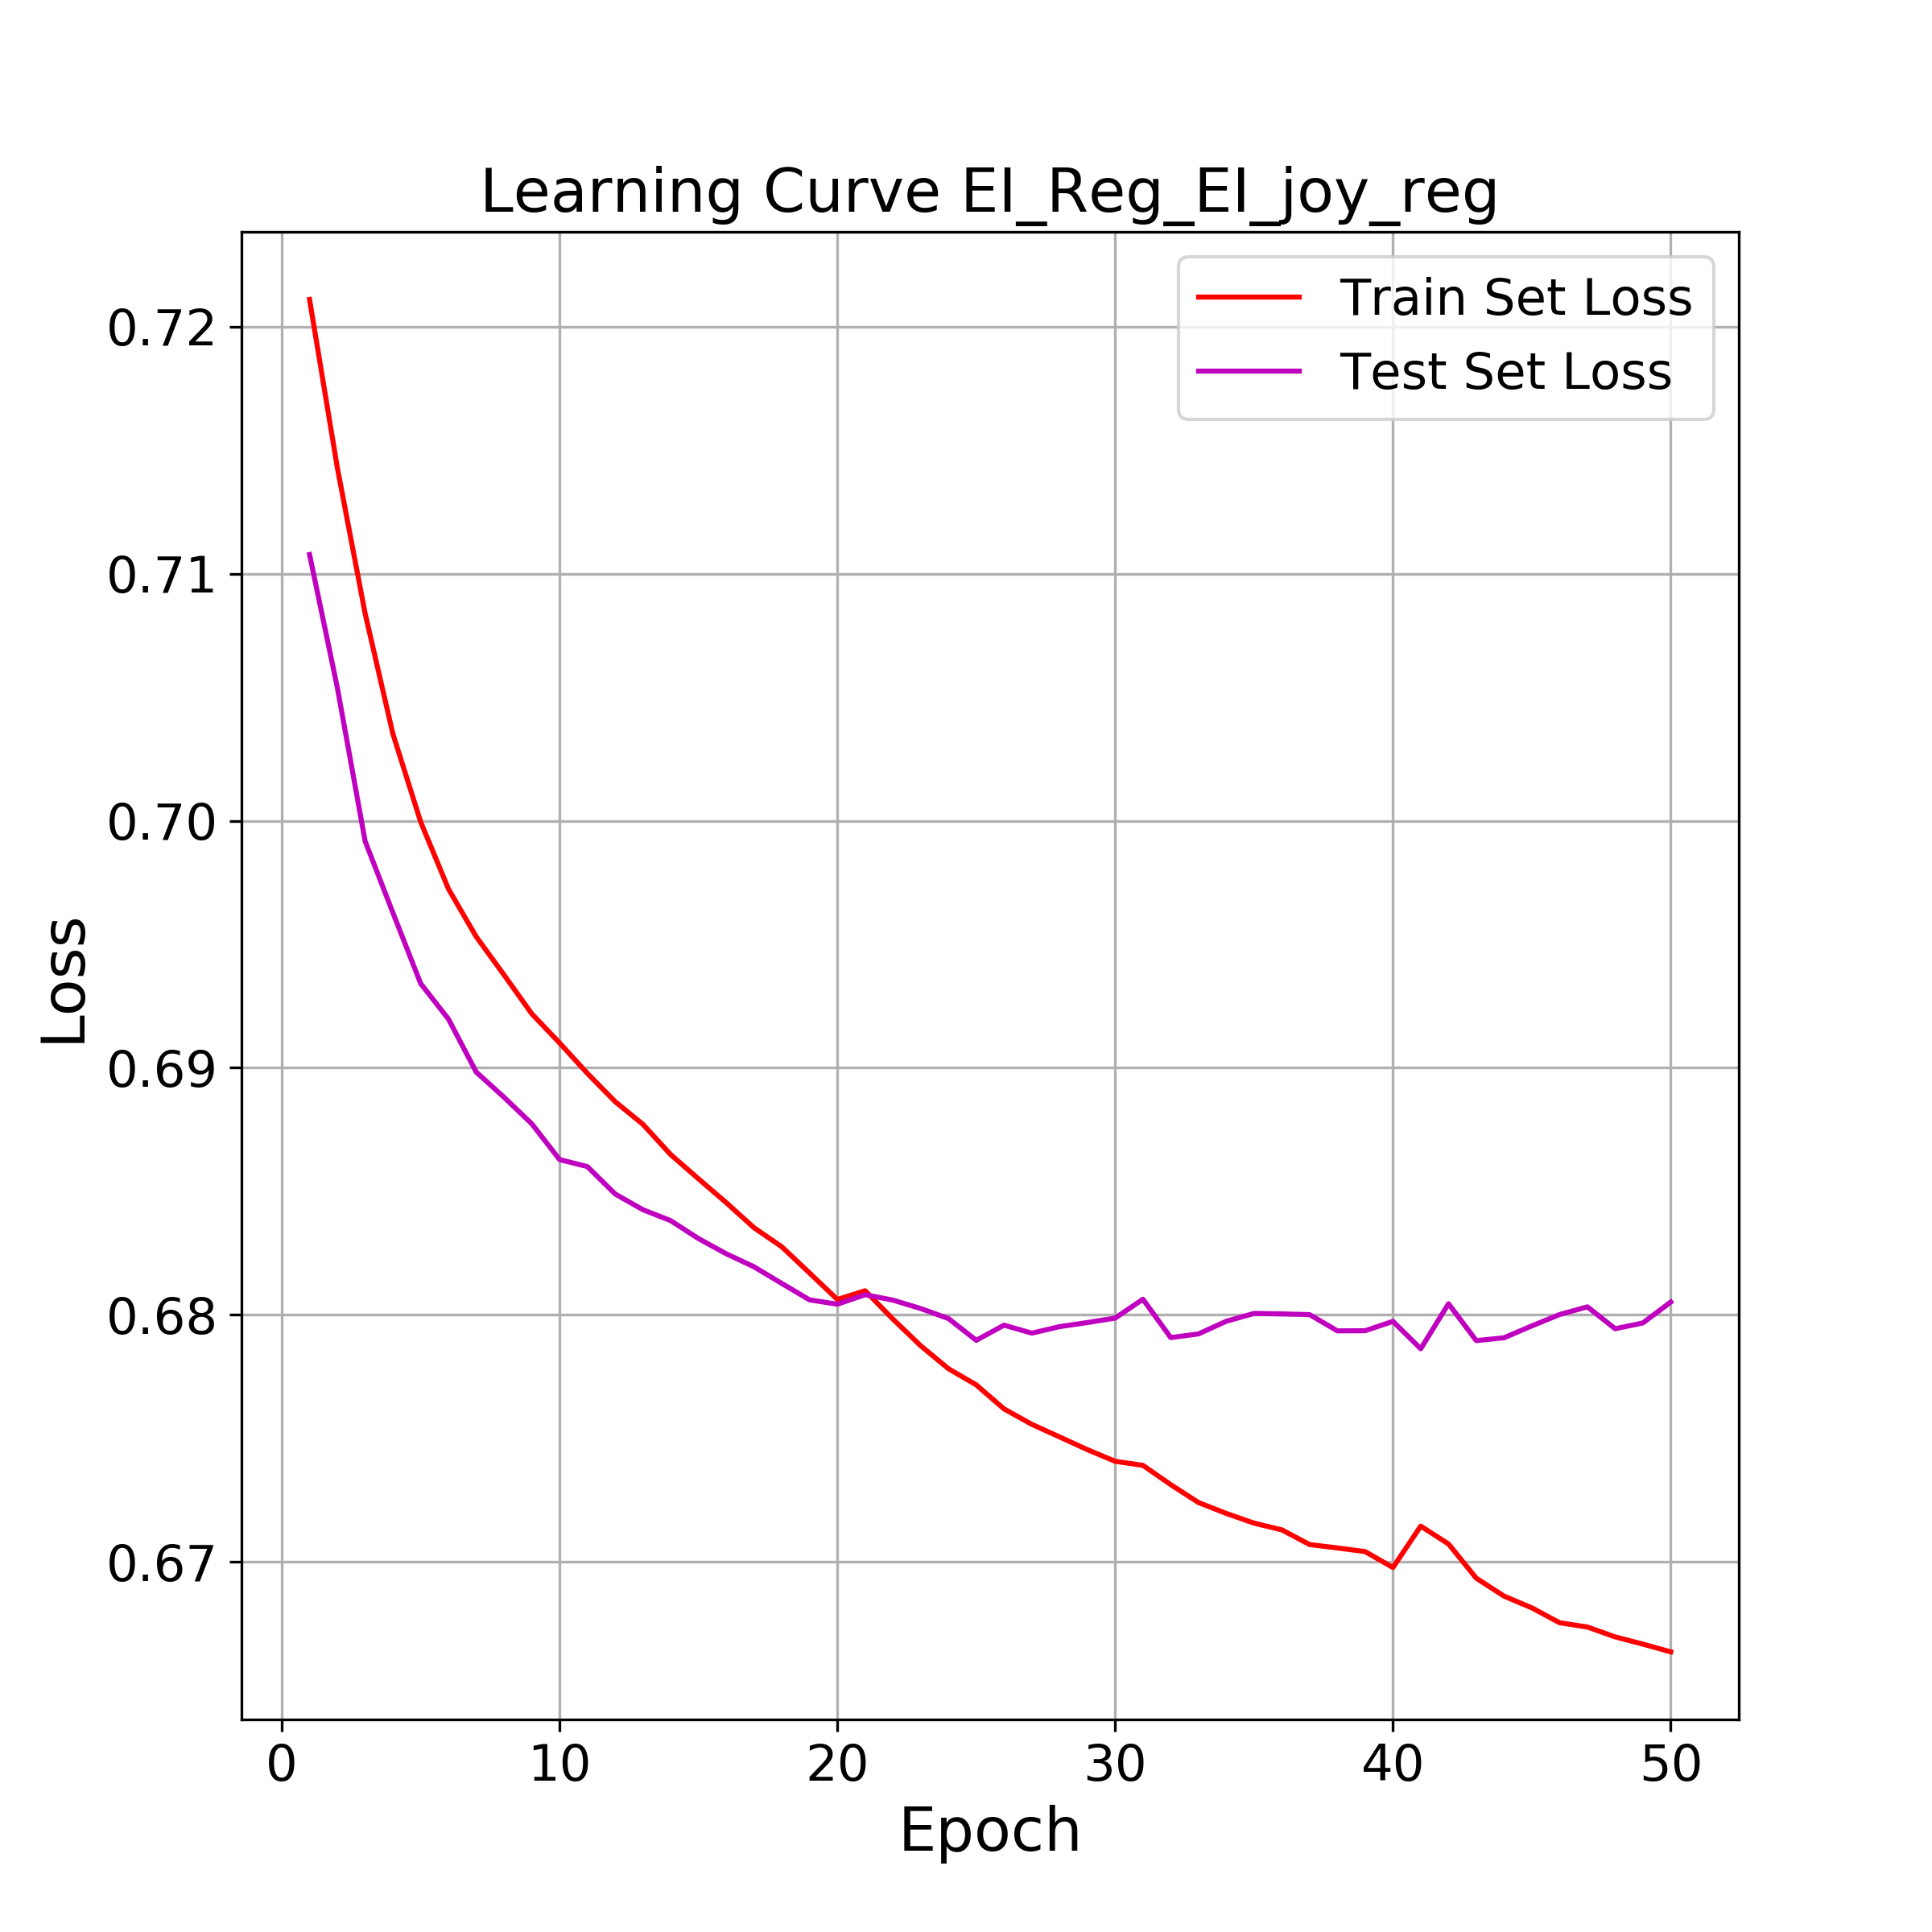
\includegraphics[width=0.6\linewidth]{./img/EI_Reg/EI_joy_reg_loss}
	\caption{Joy Learning Curve}
	\label{fig:sin}
\end{figure}

\textbf{Joy}
Min Test Loss: 0.678624
Pearson corellation coefficient r: 0.481580
\begin{figure}[h!]
	\centering
	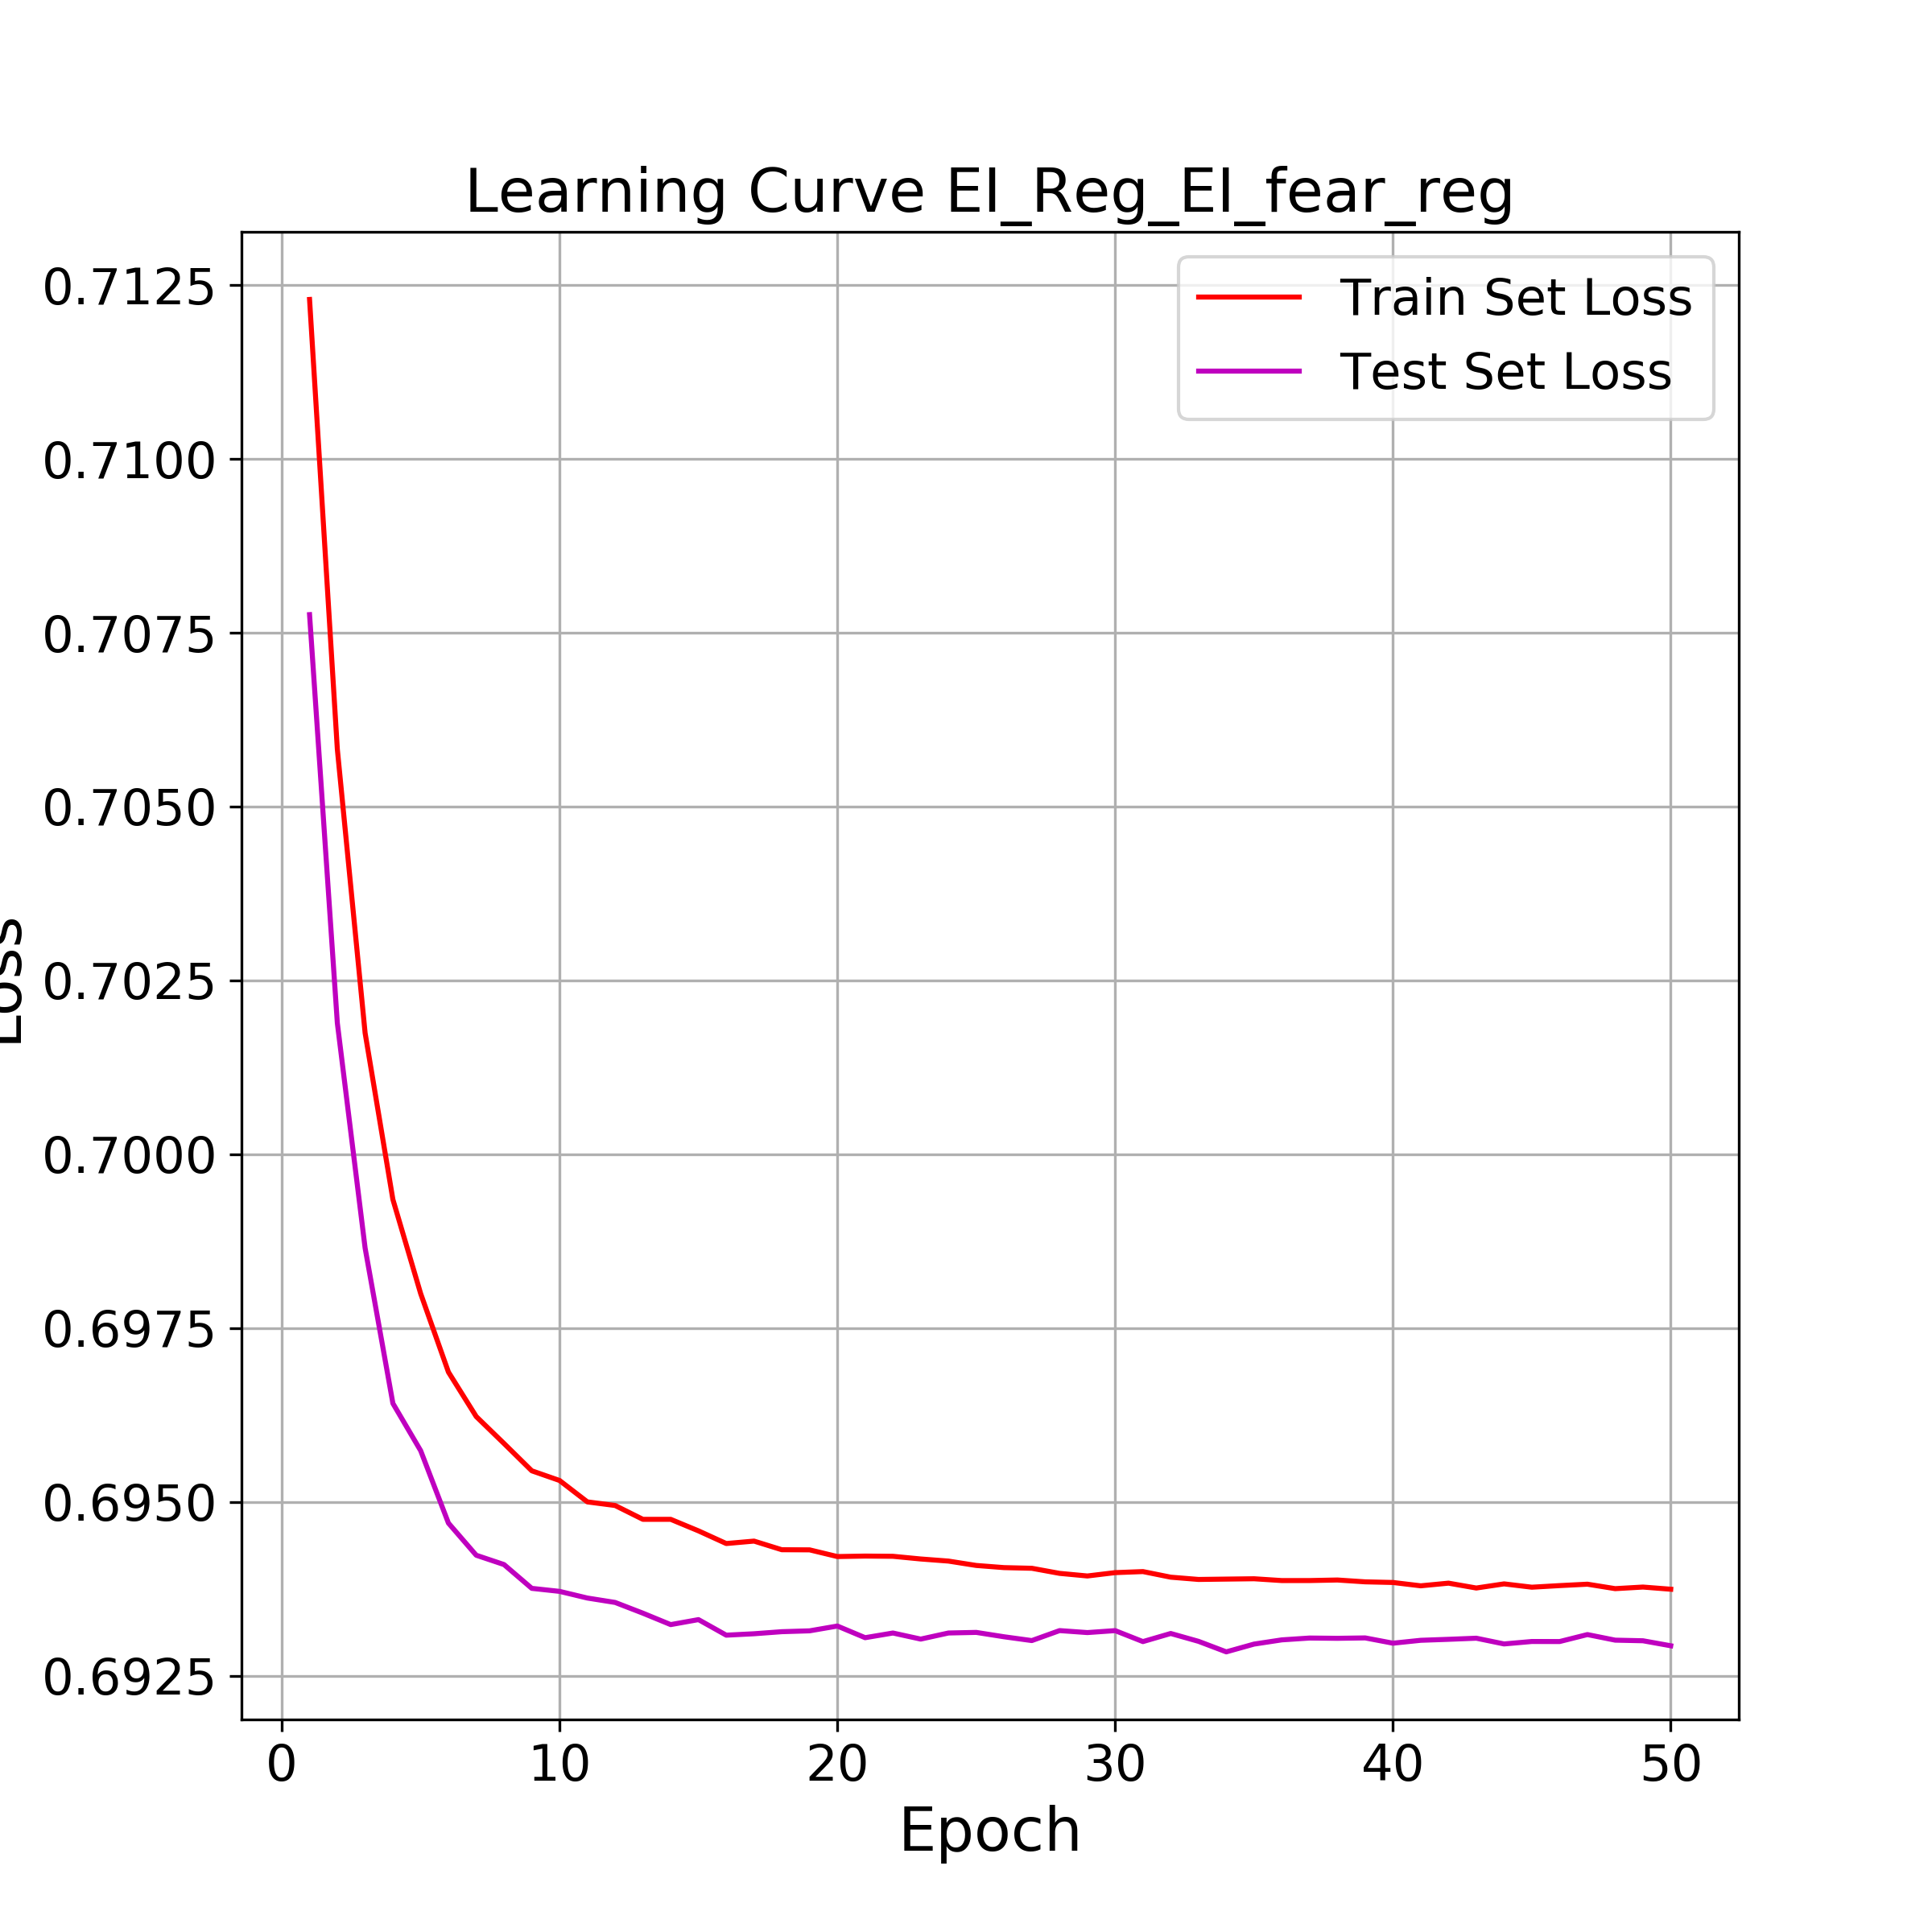
\includegraphics[width=0.6\linewidth]{./img/EI_Reg/EI_fear_reg_loss}
	\caption{fear Learning Curve}
	\label{fig:sin}
\end{figure}

\textbf{fear}
Min Test Loss: 0.692845
Pearson corellation coefficient r: 0.023532


\begin{figure}[h!]
	\centering
	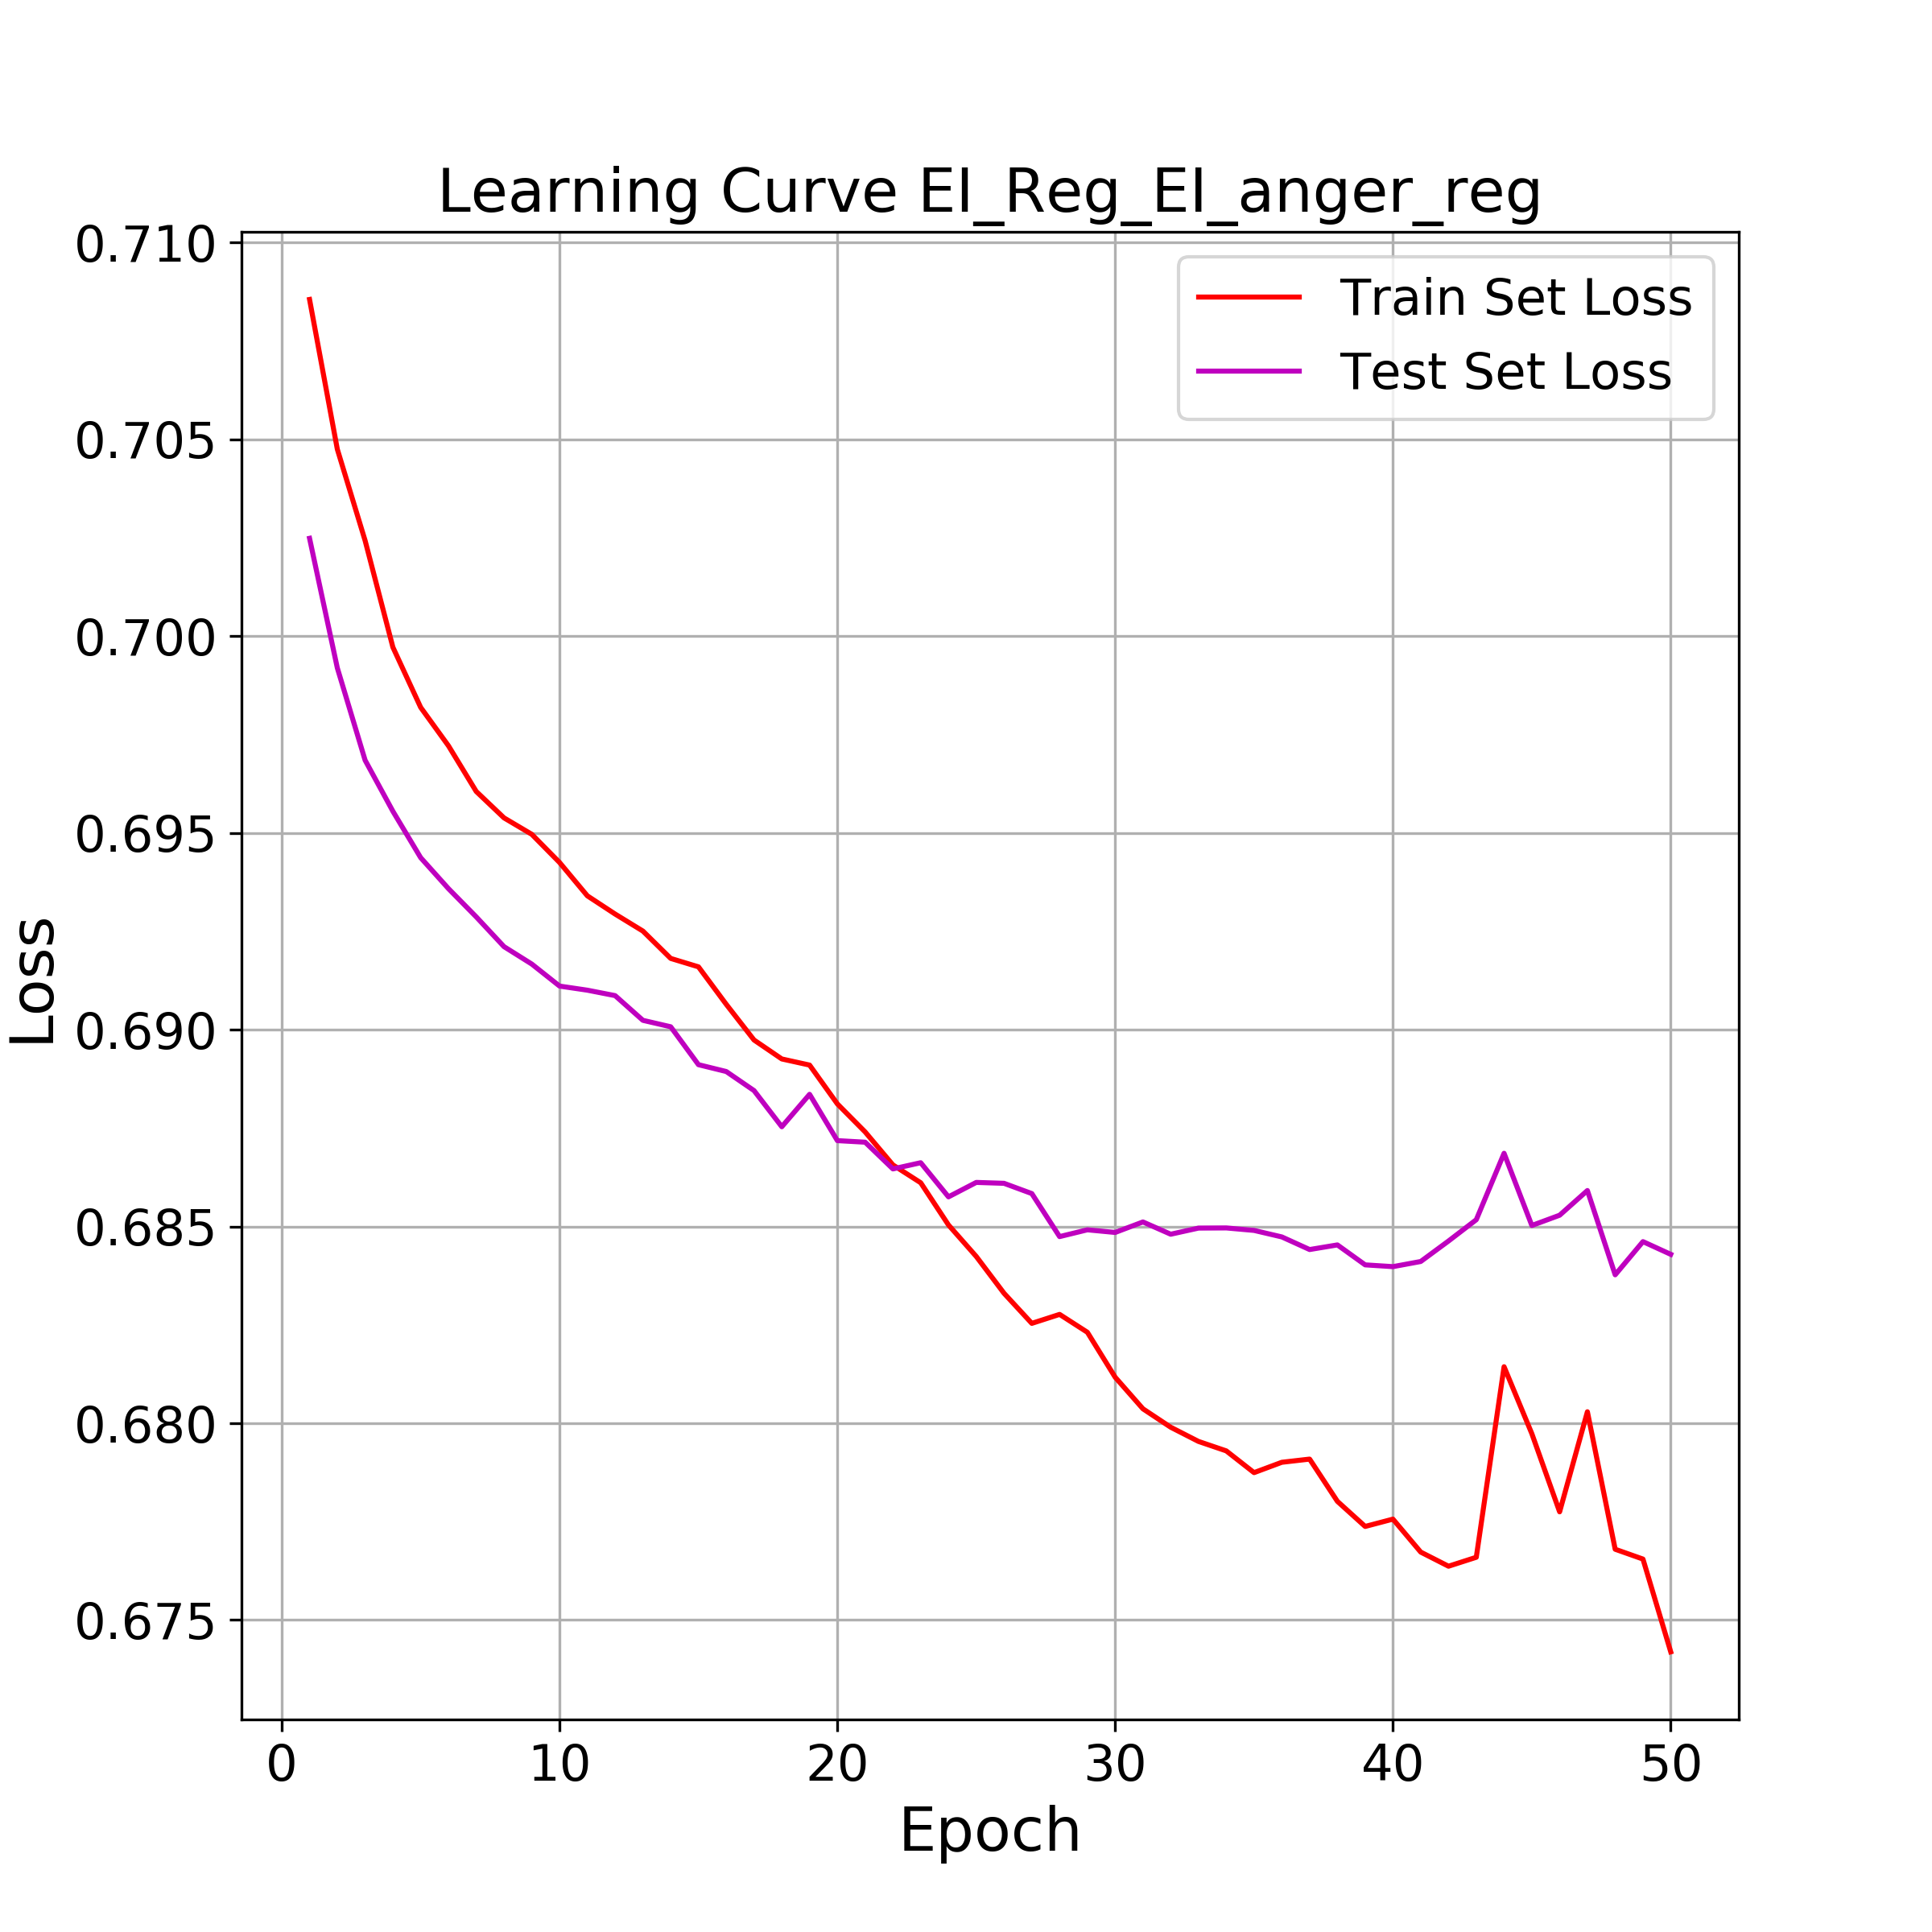
\includegraphics[width=0.6\linewidth]{./img/EI_Reg/EI_anger_reg_loss}
	\caption{anger Learning Curve}
	\label{fig:sin}
\end{figure}

\textbf{Anger}
Min Test Loss: 0.683772
Pearson corellation coefficient r: 0.360298


\begin{figure}[h!]
	\centering
	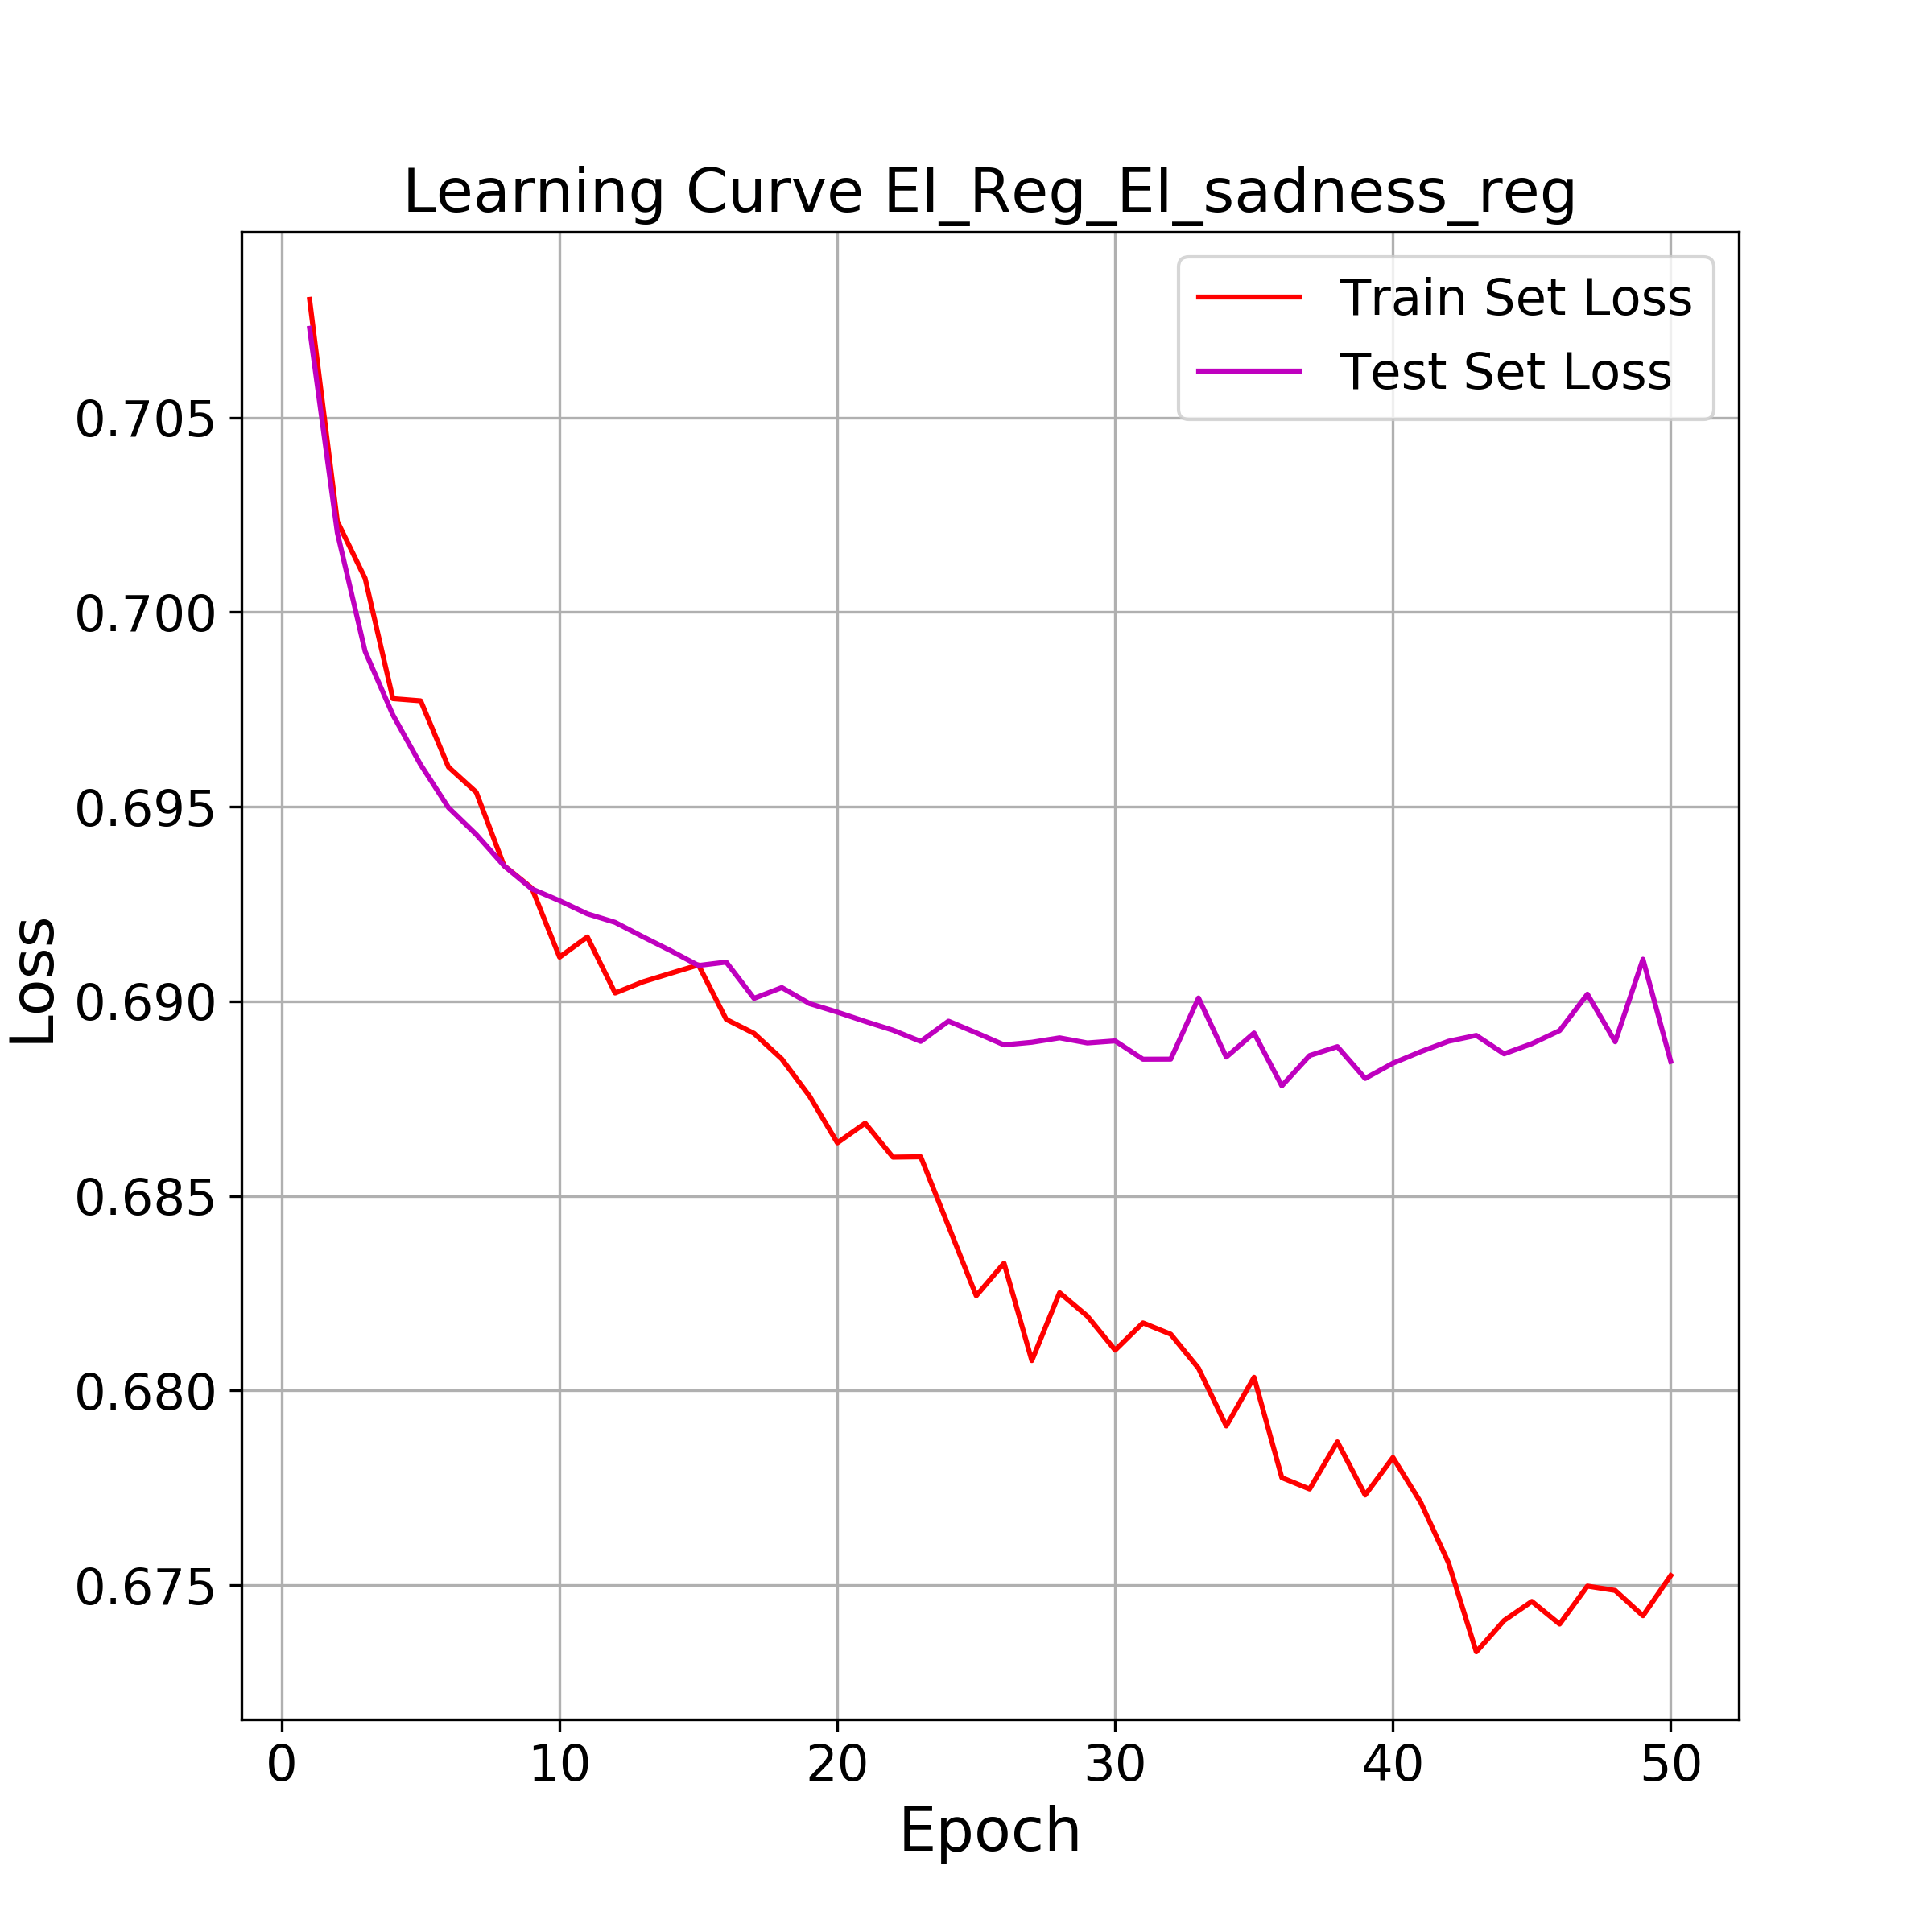
\includegraphics[width=0.6\linewidth]{./img/EI_Reg/EI_sadness_reg_loss}
	\caption{sadness Learning Curve}
	\label{fig:sin}
\end{figure}


\textbf{Sadness}
Min Test Loss: 0.687828
Pearson corellation coefficient r: 0.328348






\subsection*{References}
[1] https://pathmind.com/wiki/bagofwords-tf-idf

[2] https://nlp.stanford.edu/projects/glove/

[3] http://www.cs.cornell.edu/people/pabo/movie-review-data/

[4] http://alt.qcri.org/semeval2017/task4/index.php?id=data-and-tools


\end{document}